% --- Template for thesis / report with tktltiki2 class ---
% 
% last updated 2013/02/15 for tkltiki2 v1.02

\documentclass[english]{tktltiki2}

% tktltiki2 automatically loads babel, so you can simply
% give the language parameter (e.g. finnish, swedish, english, british) as
% a parameter for the class: \documentclass[finnish]{tktltiki2}.
% The information on title and abstract is generated automatically depending on
% the language, see below if you need to change any of these manually.
% 
% Class options:
% - grading                 -- Print labels for grading information on the front page.
% - disablelastpagecounter  -- Disables the automatic generation of page number information
%                              in the abstract. See also \numberofpagesinformation{} command below.
%
% The class also respects the following options of article class:
%   10pt, 11pt, 12pt, final, draft, oneside, twoside,
%   openright, openany, onecolumn, twocolumn, leqno, fleqn
%
% The default font size is 11pt. The paper size used is A4, other sizes are not supported.
%
% rubber: module pdftex

% --- General packages ---

\usepackage[utf8]{inputenc}
\usepackage[T1]{fontenc}
\usepackage{lmodern}
\usepackage{microtype}
\usepackage{amsfonts,amsmath,amssymb,amsthm,booktabs,color,enumitem,graphicx}
\usepackage[pdftex,hidelinks]{hyperref}
\usepackage{verbatim}
\usepackage{multicol}
\usepackage{breakurl}
\usepackage[breaklinks]{hyperref}
\def\UrlBreaks{\do\/\do-}

% Automatically set the PDF metadata fields
\makeatletter
\AtBeginDocument{\hypersetup{pdftitle = {\@title}, pdfauthor = {\@author}}}
\makeatother

% --- Language-related settings ---
%
% these should be modified according to your language

% babelbib for non-english bibliography using bibtex
\usepackage[fixlanguage]{babelbib}

% add bibliography to the table of contents
\usepackage[titletoc]{appendix}
\usepackage[nottoc,notlot,notlof]{tocbibind}


% --- Theorem environment definitions ---
\newtheorem{thm}{Theorem}
\newtheorem{lem}[thm]{Lemma}
\newtheorem{cor}[thm]{Corollary}

\theoremstyle{definition}
\newtheorem{definition}[thm]{Definition}

\theoremstyle{remark}
\newtheorem*{remark}{Remark}

\def\signed#1{{\leavevmode\unskip\nobreak\hfil\penalty50\hskip2em
  \hbox{}\nobreak\hfil\raise-3pt\hbox{(#1)}%
  \parfillskip=0pt \finalhyphendemerits=0 \endgraf}}

\newsavebox\mybox
\newenvironment{aquote}[1]
  {\savebox\mybox{#1}\begin{quotation}}
  {\signed{\usebox\mybox}\end{quotation}}

% --- tktltiki2 options ---
%
% The following commands define the information used to generate title and
% abstract pages. The following entries should be always specified:

\title{Transitioning the development process towards Continuous Delivery and Continuous Experimentation: A Case Study in the B2B Domain}
\author{Olli Rissanen}
\date{\today}
\level{Master's thesis}
\abstract{Delivering more value to the customer is the goal of many software companies. Delivering value in real-time requires a company to utizile real-time deployment of software, data-driven decisions and empirical evaluation of new products and features. Real-time deployment of software allows for faster reaction times and shorter feedback loops. Evaluating new products and features allows organizations to steer development based on quantifiable data. This thesis is an exploratory case study investigating practices known as continuous delivery and continuous experimentation to tackle real-time delivery and data-driven decisions. Continuous delivery is a development practice where the software functionality is deployed continuously to customer environment. This process includes both automated builds and automated testing, but also automated deployment. Continuous experimentation is a development practice where the entire R\&D process is guided by conducting experiments and collecting feedback. Such experiments can include deploying multiple versions of software with different properties, measuring their success based on some criteria and then selecting the best candidate for further development. This paper conducts a deductive case study in a medium-sized software company to examine the development process of two different software products, and the transition towards continuous delivery and continuous experimentation. The scope of this study is in the B2B domain, where the products are developer directly to other companies acting as customers. The research objective is to analyze the challenges, benefits and systematic organisation of continuous delivery and continuous experimentation in this domain. As a result, the challenges and best practices in the transition are identified. The results suggest that technical challenges are only one part of the challenges a company encounters in this transition. \\\newline ACM Computing Classification System (CCS): \newline \textbf{General and reference $\rightarrow$ Experimentation} \newline \textbf{General and reference $\rightarrow$ Measurement} \newline \textbf{General and reference $\rightarrow$ Validation}}

% The following can be used to specify keywords and classification of the paper:

\keywords{Continuous delivery, Continuous experimentation, Development process}

%\classification{General and reference → Experimentation}
% classification according to ACM Computing Classification System (http://www.acm.org/about/class/)
% This is probably mostly relevant for computer scientists
% uncomment the following; contents of \classification will be printed under the abstract with a title
% "ACM Computing Classification System (CCS):"
% \classification{}

% If the automatic page number counting is not working as desired in your case,
% uncomment the following to manually set the number of pages displayed in the abstract page:
%
% \numberofpagesinformation{16 pages + 10 appendix pages}
%
% If you are not a computer scientist, you will want to uncomment the following by hand and specify
% your department, faculty and subject by hand:
%
\faculty{Faculty of Science}
\department{Department of Computer Science}
\subject{Computer Science}
%
% If you are not from the University of Helsinki, then you will most likely want to set these also:
%
\university{University of Helsinki}
% \universitylong{HELSINGIN YLIOPISTO --- HELSINGFORS UNIVERSITET --- UNIVERSITY OF HELSINKI} % displayed on the top of the abstract page
\city{Helsinki}
%


\begin{document}

% --- Front matter ---

\frontmatter      % roman page numbering for front matter

\maketitle        % title page
\makeabstract     % abstract page

\tableofcontents  % table of contents

% --- Main matter ---

\newpage

It’s hard to argue that Tiger Woods is pretty darn good at what he does. But even he is not perfect. Imagine if
he were allowed to hit four balls each time and then choose the shot that worked the best. Scary good.
-- Michael Egan, Sr. Director, Content Solutions, Yahoo (Egan, 2007)

\mainmatter       % clear page, start arabic page numbering

%case study
% Relate the theory to a practical situation; for example, apply the ideas 
%and knowledge discussed in the coursework to the practical situation 
%at hand in the case study. 

%In order to improve the technical competence and to gain a deep insight on customer behavior

%In it's core continuous experimentation consists of a design-execute-analyse loop, where hypotheses are selected based on business goals and strategies, experiments are executed with partial implementations and data collection tools and finally the results are analyzed to validate the hypothesis.

\section{Introduction} %Motivation

\subsection{Overview}
To deliver value fast and to cope with the increasingly active business environment, companies have to find solutions that improve efficiency and speed. Agile practices \cite{cockburn2002agile} have increased the ability of software companies to cope with changing customer requirements and changing market needs \cite{dzamashvili2010impact}. To even further increase the efficiency, shortening the feedback cycle enables faster customer feedback. Additionally, providing software functionality to collect usage data can be used to guide the product development and to increase the value generated for customers. Eventually the company running the most and fastest experiments outcompetes others by having the data to develop products with exceptional qualities \cite{eklund2012architecture}.

The requirement of developing value fast has led to the evolution of a new software development model \cite{bosch2012building}. The model is based on three principles: evolving the software by frequently deploying new versions, using customers and customer data throughout the development process and testing new ideas with the customers to drive the development process and increase customer satisfaction. Currently more and more software companies are transitioning towards this model, called innovation experiment systems. 

The logical starting point of this thesis was an open issue by the case company: how do we validate whether a feature would be succesful or not? To provide an answer to this question, two software development models known as continuous delivery and continuous experimentation are analyzed as possible development models for the case company. 
%The whole pipe between the idea and implementation isn't yet completely perceived. Some parts are visible, but the entirety is still unclear.

%-this creates barriers
%-Delivering value in real-time
%  -requires: real-time delivery
%  -requires: empirically evaluating new products and services
%-Deep customer insights
%  -data-informed solutions
%  -a deep understanding of customers and products by gathering data continuously from the live use of the products.
%-Interesting aspects:
%-Products with a history cannot be developed in a MVP manner, more like in a MVF (feature) manner.
%IEEE divides the quality of a software component into two components: how well the software meets software requirements specifications, and how useful the software is to the end user.
%CMMI 5th stage 

Continuous delivery is a way to shorten the delivery cycles and to automate the delivery process is. It is an extension to continuous integration, where the delivery process is often entirely automated, and software functionality is deployed frequently to customer environment. While continuous integration defines a process where the work is automatically built, tested and frequently integrated to mainline \cite{fowler2006continuous}, often multiple times a day, continuous delivery adds automated acceptance testing and deployment. Continuous delivery therefore attempts to deliver an idea to users as fast as possible by automating the deployment process.

In continuous experimentation model the organisation continuously executes controlled experiments to guide the R\&D process. The process of guiding R\&D through experiments is used to validate that an idea is, in fact, a good idea. The development cycle in continuous experimentation resembles the Build-Measure-Learn cycle of Lean Startup \cite{ries2011lean}. The process in continuous experimentation is to first form a hypothesis based on a business goals and customer "pains" \cite{bosch2012building}. After the hypothesis has been formed, quantitative metrics to measure the hypothesis must be decided. After this a minimum viable product can be developed and deployed, while collecting the required data. Finally, the data is analyzed to validate the hypothesis.

Fagerholm et al. define that a suitable experimentation system must be able to release minimum viable products or features with suitable instrumentation for data collection, design and manage experiment plans, link experiment results with a product roadmap and manage a flexible business strategy \cite{fagerholm2014building}. The Build-Measure-Learn cycle starts with forming a hypothesis and building a minimum viable product (MVP) with tools for data collection. Once the MVP has been created, the data is analyzed and measured in order to validate the hypothesis. To persevere with a chosen strategy means that the experiment proved the hypothesis correct, and the full product or feature can be implemented. However, if the experiment proved the hypothesis wrong, the strategy is changed based on the implications of a false hypothesis.

In the context of this thesis, continuous experimentation refers to a development model following these principles: 
\begin{itemize}
\item  Data driven decisions
\item  Link product development and business aspect
\item  React to customers present needs
\item  Turn hypotheses into facts
\item  Steer development process
\end{itemize}

Many development models that carry a different name share the key principles with continuous experimentation. One of such is the innovation experiment system \cite{bosch2012building}. It is a development model where the development process consists of frequently deploying new versions and using customers and customer usaged data in the development process \cite{bosch2012building}. The model focuses on innovation and testing ideas with customers to drive customer satisfaction and revenue growth \cite{bosch2012building}. "First, it frequently deploys new versions focusing on continuously evolving the embedded software in short cycles of 2-4 weeks" \cite{eklund2012architecture}.

%In this thesis we conduct a case study to analyse the adoption of continuous deployment and continuous experimentation in B2B domain. The case study consists of a literature review on applications of these practices, an interview of key members in the case company and analysis of the results. 

This study is an exploratory deductive case study, which aims to explore how continuous delivery and continuous experimentation can be applied in the case company. While existing studies of applying the development models exist, none of the studies focuses specifically in the B2B domain. This study specifically aims to identify the main requirements, problems and key success factors with regards to these approaches. Integrating these approaches to the development process requires a deep analysis of the current development process, seeking the current problems and strengths. Adopting both continuous delivery and continuous experimentaton also requires understanding the requirements of continuous delivery and continuous experimentation, and restrictions caused by the developed software products. 

In this research, the units under the study are two teams and two different software products developed by each team. By focusing on different products, a broader view on the application of these development approaches can be gained. The other product, a marketing automation called Dialog, is used through an extensive user interface. The other product under inspection is CDM, a Master Data Management \cite{loshin2010master} solution running as an integrated background application. The objective of this thesis can therefore be summarized as follows:

\bigskip
\noindent \textbf{Research objective}
To analyze the software development process transition towards shorter feedback cycle and data-driven decisions from the perspective of the case company, with respect to continuous delivery and continuous experimentation practices.

\subsection{Research questions}

The broader research objective is explored here. The research questions are structured to progress from a higher-level perspective to a more detailed view. The first two research questions are needed to study the requirements and benefits of these practices to rationalize the decisions to embrace these practices. Then, the third research question corresponds to the operational adjustments required to adopt these practices. \newline

%Literature review / Interview
\noindent \textbf{RQ1: What are the B2B specific challenges of continuous delivery and continuous experimentation?}

\noindent Software development practices and product characteristics vary based on the domain and delivery model. Typical B2C applications are hosted as SaaS applications, and accessed by users via a web browser. In the B2B domain, applications installed to customer environments are very common. Running experiments on customer environments also requires a new deployment of the software product, possibly causing downtime and changing some functionality of the software. The purpose of this research question is to identify the challenges in these practices in the B2B environment. The research question is answered by conducting an interview to discover B2B specific challenges, and using the available literature on continuous delivery and continuous experimentation to draw conclusions on the environmental differences.
%Question: contractual issues? 
%Question: selecting the correct OEC in b2b is harder. for example revenue. 
%question: in B2C people develop their own product, but in B2B the feature ideas might come only from customer.
\newline

%collect ideas from literature review and interview
%\noindent \textbf{RQ 2: How to collect usage data and customer feedback in B2B domain, where user amounts can be very low?}

%\noindent Research question 4 is answered by analysing the usage data and customer feedback collection of the case company. This is carried out by interviewing the key persons responsible for customer interaction and developers responsible for usage data collection.  

%As compared to the B2C domain where the product is often deployed in cloud with a lot of users, B2B applications might only have a handful of users. This question %is answered by collecting ideas from the literature review and interview results. \newline
%-Legal issues
%-Technical issues

%Interview results have to be compared to literature review results
\noindent \textbf{RQ2: How do continuous delivery and continuous experimentation benefit the case company?} %What are the problems and strengths of the current development process?

\noindent To rationalize the decision to adopt continuous delivery and experimentation in a company, the actual benefits to the business have to be identified. This research question aims to identify clear objectives for what should be achieved with continuous delivery and continuous experimentation. Sections of the interview aim to identify the current perceived problems of the case company related to deployment, product development, collecting feedback and guiding the development process. These problems are then compared to the benefits of these approaches found from the literature review, taking into account the challenges identified in RQ1.
\newline

%When you
%present the vision to these stakeholders it is important to have
%the mission clarified. What are you trying to achieve through
%continuous delivery and why? You must set clear objectives
%and keep progress steering toward the right direction. There
%are many side paths, experiments and “shiny” things to distract
%you on the journey towards continuous delivery. It is easy to
%become distracted or waylaid by these.

%\noindent \textbf{RQ 3: What is the Minimum Viable Process of continuous experimentation?}

%\noindent While a definitive process of continuous experimentation hasn't been defined, a process with multiple different roles is quite heavyweight and not quickly adoptable. The purpose of this research question is to identify the core practices and requirements of continuous experimentation. How can the process be kept as simple as possible without losing the benefits? The goal is that companies are able to quickly test whether the process suits their needs. This requires that the process is defined in such level of abstraction that it can be adopted in practice with relative ease. This research question is answered based on literature %review. To answer this research question, a deep understanding of the process has to be established. \newline

%collect ideas from literature review and interview
\noindent \textbf{RQ3: How can continuous experimentation be systematically organised in the B2B domain?}

\noindent When the benefits and requirements are identified and the process is decided to be approved by a company, it has to be adopted and applied in practice. This research question investigates how to apply these practices in the case company, and aims to answer to questions such as what, how, who and when. This question is answered by applying Fagerholm et al. model \cite{fagerholm2014building} to two different teams and software products within the case company, and addressing the challenges found in the first research question. Then the deviations in the model are identified, and possible solutions to these deviations provided. \newline
%-Where do the feature ideas come from?
%-What roles are required?

\subsection{Scope and limitations}
This study focuses on the development process of the case company and its two software products in the B2B domain. Case studies only allow analytic generalisations, and the findings cannot be directly generalised to other cases. This limitation applies especially to applying continuous delivery and continuous experimentation in practice, since software products and customers inevitably differ. The background theory is drawn from literature focusing on continuous delivery, continuous experimentation, Lean Startup and innovation experiment systems. 

The empirical research of this thesis has been carried out in the context of a medium sized information technology company, Steeri Oy. The company specializes in customer data on multiple fronts: CRM, BI, Master Data Management and data integrations, among others. The empirical research has applied case study methodology to offer deep understanding of the phenomena in their natural context. The tradeoff of a case study research is that it does not provide much room for direct generalizations outside the empirical context. 

This thesis is organized as follows. The first chapter is the introduction at hand. The second and third chapter summarize the relevant literature and theories to position the research and to educate the reader on the body of knowledge and where the contributions are intended. The fourth chapter briefly explains the usage of case study and qualitative research as research methods, to provide background for the decision to utilize them in this particular study. The fifth chapter presents the research design: objectives, context and applied methods. The findings are then presented in the sixth chapter, organized according to the research questions. The seventh chapter summarizes and interprets the main results, and discusses the limitations of the thesis. Finally, the eight chapter summarizes the thesis by explaining the contributions to current research and introducing further research avenues.
%Structure:
%
%#1
%Background information - case study context - results - limitations - summary, future work
%#2
%Related work - experimental setup - results - summary
%-GOAL OF THE THESIS
%-motivation
%-research question
%-approach
%>analyze state of the practice
%>specify problem and goals 
%>analyze state of the art
%>state hypotheses
%>derive solution idea

\subsection{Contributions}
This thesis contributes to continuous experimentation \cite{fagerholm2014building} and organization evolution path \cite{olsson2012climbing} discussions by analysing the theories in B2B domain. These research areas are increasingly interesting in research, but none of the existing studies focuses purely on the B2B domain. There is growing research interest in these areas, however, most of the research takes place in B2C domain. Thus, the primary contribution of this thesis is to analyze the effects of this phenomena in a new domain. 

The research objective of this thesis included the analysis of both continuous delivery and continuous experimentation. The third research question focuses only on continuous experimentation, as the attempt to study both approaches simultaneously would have required the analysis of too many variables at once. 

This research contributes to continuous delivery research by identifying issues found when the software is produced for customer companies. The study suggests that the challenges faced in the B2B context are multidimensional, and related to the technical, procedural and customer aspects. The primary issues causing these challenges are the customer owned environment and the importance of the software product for the customer. However, the study also suggests that continuous delivery corresponds to many of the case company's primary needs, such as improving the reliability of versions and reducing the time required for deploying versions.

The contributions to continuous experimentation research are firstly identifying the challenges a company faces in the transition towards an experimental system. These challenges are examined by utilizing two different software products, to provide two different perspectives. Secondly, the benefits of continuous experimentation are mapped to actual needs by the case company. Thirdly, an initial continuous experimentation infrastructure \cite{fagerholm2014building} is mapped to the case company's context with the required deviations.
\section{Literature: Continuous Delivery}
%Agile
Software development models have been moving towards shorter feedback loops since iterative software development methods. Agile software development emerged from the iterative software development methods, with early implementations being development in the 1990's \cite{dybaa2008empirical}. The general principles of agile software development are breaking the development to short iterations, maintaining a short feedback loop with the customer by having a customer representative, valuing working software over documentation and responding to change. The highest agile principle is to satisfy the customer through early and continuous delivery of software. Continuous delivery therefore has its roots in agile software development. Many agile models, such as Scrum \cite{schwaber2002gile}, Extreme Programming \cite{beck2000extreme} and Feature-Driven Development \cite{palmer2001practical} further define their own strategies based on the agile principles. Scrum, for example, defines a framework for managing product development, without much focus on technical tools. Extreme Programming, on the other hand, includes many technical features, such as always programming in pairs, doing extensive code review and unit testing.

%Lean manufacturing & LSD
Continuous delivery has also been influenced by Lean manufacturing, which is derived from the Toyota Production System \cite{ono1988toyota}. Lean manufacturing is a streamlined production philosophy that aims to identify the expenditure of resources not used in creating value for the end customer, and eliminate these activities. Lean software development \cite{poppendieck2003lean} has been developed based on the same idea. The purpose of lean software development is to eliminate waste, or anything that doesn't bring value to the customer, and to pursue perfection through smoothing the development flow. The principles in lean software development are eliminate waste, amplify learning, decide as late as possible, deliver as fast as possible, engage everyone, create quality and see the whole. 

Lean software development, developed based on the lean manufacturing principles, is a development approach attempting to eliminate unnecessary work and to create value for the customer. Lean Startup \cite{ries2011lean} is a method for developing products based on the lean software development principles. The key component of Lean Startup is the Build-Measure-Learn loop, which guides the development process by defining a loop process where ideas are turned into products, which are then measured and the idea pivoted or persevered forwards.

%Lean startup
The software development models have moved towards even shorter and shorter feedback loops in the recent years. A primary purpose of Lean Startup is to assess the specific demands of consumers and to fulfill those demands with the least possible resources. The Build-Measure-Learn loop is used to learn the customers actual needs and consecutively to steer business and product strategies to the correct direction. The tight customer feedback loop ensures that the product development doesn't include features and services not wanted by the customer. 

Continuous delivery is a design practice where the software delivery process is automated, and thus the software can be deployed on short notice. Olsson et al. have investigated the evolution path of software companies, and have identified continuous delivery and "R\&D as an Experiment System" as final stages \cite{olsson2012climbing} of the evolution path. Continuous delivery is also seen as a prerequisite for continuous experimentation, as it provides a way to quickly deploy new features. 

\begin{figure}[h]
	\centering
	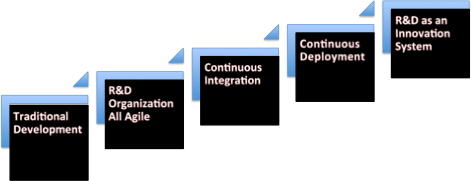
\includegraphics[width=5.0in]{stairway.png}
	\caption{Organization evolution path \cite{olsson2012climbing}.}
\end{figure}

In this chapter we first introduce the general principles of continuous delivery and continuous deployment. Then we introduce the software deployment pipeline and the effects of continuous delivery on the development model. Finally, we list challenges faced when applying continuous delivery.

%The most important idea behind continuous delivery is to deliver an idea to the customer as fast as possible.  

%-Stairway to heaven
%-Innovation experiment system

%\subsection{Development pipeline}

\subsection{Continuous delivery}

To be able to react to customers changing requests and manage multiple customer environments, the software product has to be deployed frequently and with different configurations. As the case company is working in an agile manner, requests change and adjust often. To improve the software product, the case company has a need for a deployment approach that has the following benefits:

\begin{itemize}
\item Fast feedback on changes
\item Automation of repetitive actions
\item Validating that deployed code has passed automated tests 
\item Traceable. large history records and changelogs
\item Configurable per customer environment
\end{itemize}

Fast feedback is used to validate the functionality of the software and to ensure that quality requirements are met. Automation of repetitive actions ensures that the actions are performed exactly as instructed, without room for manual error. Reducing the amount of manual work also improves efficiency. With traceable history records, troubleshooting process can be shortened. With changelogs, the customer can be kept informed of the changes in new versions. A design practice that fills the aforementioned benefits is continuous delivery.

%what is it
Continuous delivery is an extension to continuous integration, where the software functionality is deployed frequently at customer environment. While continuous integration defines a process where the work is automatically built, tested and frequently integrated to mainline \cite{fowler2006continuous}, often multiple times a day, continuous delivery adds automated acceptance testing and deployment to a staging environment. The purpose of continuous delivery is that as the deployment process is automated, it reduces human error, documents required for the build and increases confidence that the build works \cite{cdbook}. 

%release cycles
In an agile process software release is done in periodic intervals \cite{cockburn2002agile}. Compared to waterfall model it introduces multiple releases throughout the development. Continuous delivery, on the other hand, attemps to keep the software ready for release at all times during development process \cite{cdbook}. Instead of stopping the development process and creating a build as in an agile process, the software is continuously deployed to customer environment. This doesn't mean that the development cycles in continuous delivery are shorter, but that the development is done in a way that makes the software always ready for release.
\begin{figure}[h]
	\centering
	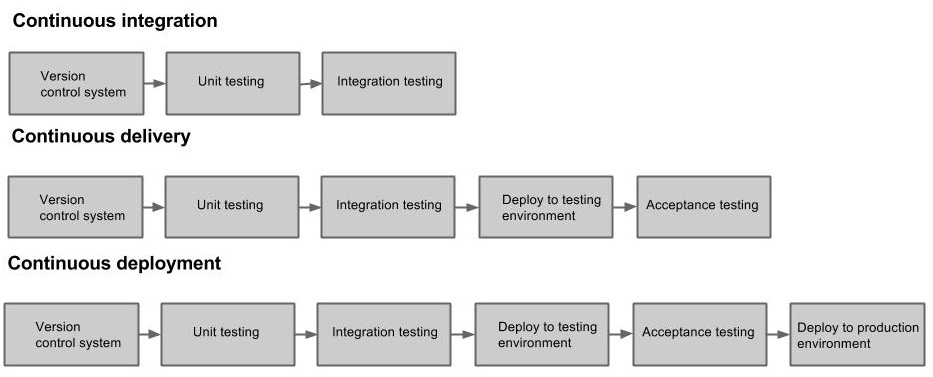
\includegraphics[width=5.0in]{rtvd.jpg}
	\caption{Continuous integration, delivery and deployment.}
	\label{fig1}
\end{figure}
%delivery vs deployment
Continuous delivery differs from continuous deployment. Refer to Fig. \ref{fig1} for a visual representation of differences in continuous integration, delivery and deployment. Both continuous delivery and continuous deployment include automated deployment to a staging environment. Continuous deployment includes deployment to a production environment, while in continuous delivery the deployment to a production environment is done manually. The purpose of continuous delivery is to prove that every build is deployable \cite{cdbook}. While it necessarily doesn't mean that teams release often, keeping the software in a state where a release can be made instantly is often seen beneficial.

%Barriers in CI->CD transition: stairway
Holmström Olsson et al. have researched the transition phase from continuous integration to continuous delivery, and have identified barriers that companies need to overcome to achieve the transition \cite{olsson2012climbing}. One such barrier is the custom configuration at customer sites. Maintaining customized solutions and local configurations alonside the standard configurations creates issues. The second barrier is the internal verification loop, that has to be shortened not only to develop features faster but also to deploy fast. Finally, the lack of transparency and getting an overview of the status of development projects is seen as a barrier.

Olsson et al. define continuous deployment as a step in the typical evolution path for companies \cite{olsson2012climbing}. The practice of deploying versions continuously allows for faster customer feedback, ability to learn from customer usage data and to focus on features that produce real value for the customer. The authors state that in order to shorten the internal verification loop, different parts in the organization should also be involved, especially the product management as they are the interface to the customer \cite{olsson2012climbing}. They also note that finding a pro-active lead customer is essential to explore and form a new engagement model.

\subsubsection{Deployment pipeline}
An essential part of continuous deployment is the deployment pipeline, which is an automated implementation of an application's build, deploy, test and release process \cite{cdbook}. A deployment pipeline can be loosely defined as a consecutively executed set of validations that a software has to pass before it can be released. Common components of the deployment pipeline are a version control system and an automated test suite.

Humble and Farley define the deployment pipeline as a set of stages, which cover the path from a committed change to a build \cite{cdbook}. Refer to Fig. \ref{fig2} for a graphical representation of a basic deployment pipeline. The commit stage compiles the build and runs code analysis, while acceptance stage runs an automated test suite that asserts the build works at both functional and nonfunctional level. From there on, builds to different environments can be deployed either automatically or by a push of a button.

Humble et al. define four principles that should be followed when attempting to automate the deployment process \cite{humble2006deployment}. The first principle states that "Each build stage should deliver working software". As software often consists of different modules with dependencies to other modules, a change to a module could trigger builds of the related modules as well. Humble et al. argue that it is better to keep builds separate so that each discrete module could be built individually. The reason is that triggering other builds can be inefficient, and information can be lost in the process. The information loss is due to the fact that connection between the initial build and later builds is lost, or at least causes a lot of unnecessary work spent in tracing the triggering build. 

The second principle states that "Deploy the same artifacts in every environment". This creates a constraint that the configuration files must be kept separate, as different environments often have different configurations. Humble et al. state that a common anti-pattern is to aim for 'ultimate configurability', and instead the simplest configuration system that handles the cases should be implemented.
\begin{figure}[h]
	\centering
	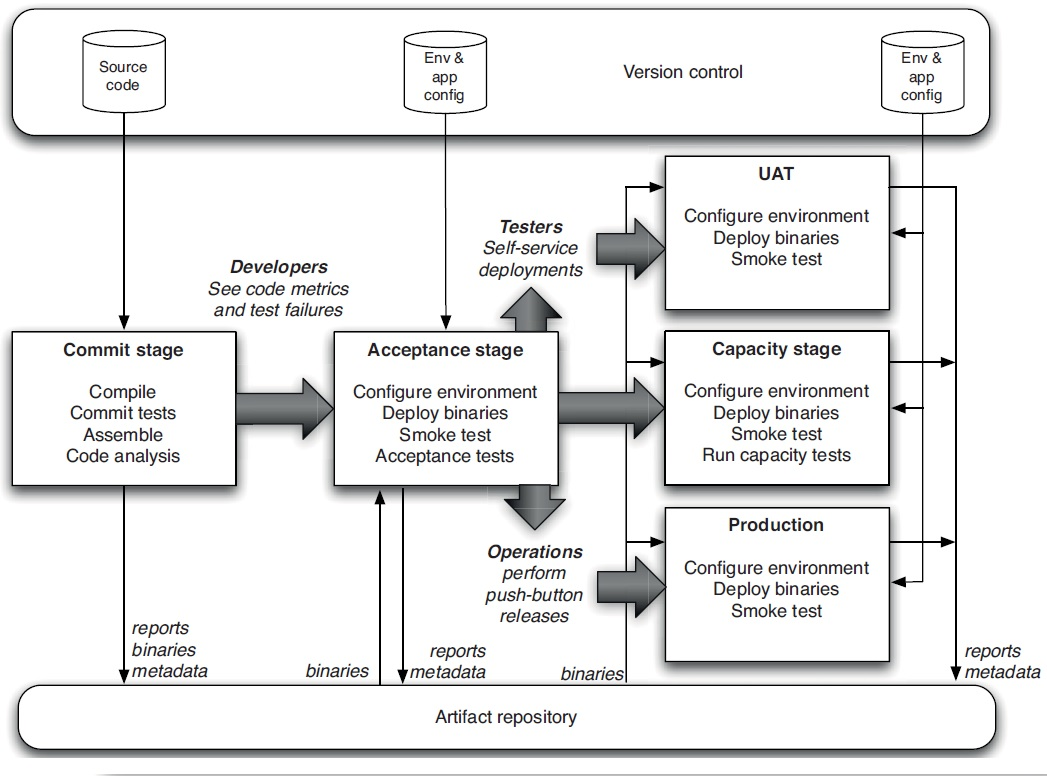
\includegraphics[width=5.0in]{pipeline.jpg}
	\caption{A basic deployment pipeline \cite{cdbook}.}
	\label{fig2}
\end{figure}
Another principle, which is the main element of continuous deployment, is to "Automate testing and deployment". Humble et al. argue that the application testing should be separated out, such that stages are formed out of different types of tests. This means that the process can be aborted if a single stage fails. They also state that all states of deployment should be automated, including deploying binaries, configuring message queues, loading databases and related deployment tasks. Humble et al. mention that it might be necessary to split the application environment into $slices$, where each slice contains a single instance of the application with predetermined set of resources, such as ports and directories. $Slices$ make it possible to replicate an application multiple times in an environment, to keep distinct version running simultaniously. Finally, the environment can be smoke tested to test the environments capabilities and status.

The last principle states "Evolve your production line along with the application it assembles". Humble et al. state that attempting to build a full production line before writing any code doesn't deliver any value, so the production line should be built and modified as the application evolves. 

\subsubsection{Impact on development model}

A picture of the typical development process in continuous delivery is shown in Fig. \ref{fig3}. After the team pushes a change to the version control system, the project is automatically built and tests are triggered stage by stage. If a test stage fails, feedback is given and the deployment process effectively cancelled. In a continuous delivery process, the last stages are approved and activated manually, but in a continuous deployment process the last stages are triggered automatically as well.

\begin{figure}[h]
	\centering
	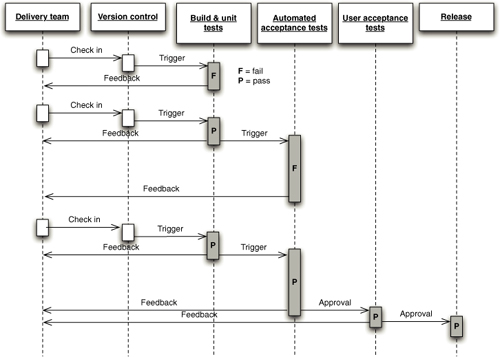
\includegraphics[width=5.0in]{developmentprocess.jpg}
	\caption{Components of the development process \cite{cdbook}.}
	\label{fig3}
\end{figure}

TODO: jatkoa tähän?

\subsection{Challenges regarding continuous delivery}
%"With continuous flow, Sales and Marketing were not quite sure when anything would be released."\cite{neely2013continuous}
% "We had to provide mechanisms where they could track the status of work in real time, so they can plan accordingly." \cite{neely2013continuous}
Neely and Stolt found out that with a continuous flow, Sales and Marketing departments lost the track of when features are released \cite{neely2013continuous}. Continuous delivery requires the company as a whole to understand the continuous flow process. Neely and Stolt solved this challenge by providing mechanisms by which the parties in need of knowledge regarding release times could track the work in real time \cite{neely2013continuous}. 

One of the largest technical challenges is the test automation required for rapid deploying \cite{humble2006deployment, cdbook}. The automated tests are often divided into multiple independend testing stages. Humble et al. note that automating the tests provide immediate value when implemented in the early stages of a project. It can, however, be a daunting task for larger projects in matured stages. Humble and Farley also bring up that implementing automated acceptance testing can be expensive and laborious, especially if communication inside the team is not effective \cite{cdbook}. 

Implementing the deployment infrastructure also requires knowledge from the development and operations team \cite{cdbook}. If the operations team doesn't understand the deployment process, the risk of making errors increases. Along with the technical implementationg, training and educating developers and operations team on the subject might be necessary depending on the prior knowledge levels.

Another challenge is to sell the vision and reasoning behind continuous delivery to the executive and management level \cite{neely2013continuous}. Neely and Stolt state that it is important to set clear objectives for what the company is trying to achieve through continuous delivery. The authors also comment that there are many "shiny" that might cause distraction on the journey towards continuous delivery. 

%It is important to have the right level of sponsorship before
%you begin. A champion trumpeting the the horn for continuous
%delivery is a key starting point but you must garner buy-in
%from the executive and senior management teams. When you
%present the vision to these stakeholders it is important to have
%the mission clarified. What are you trying to achieve through
%continuous delivery and why? You must set clear objectives
%and keep progress steering toward the right direction. There
%are many side paths, experiments and “shiny” things to distract
%you on the journey towards continuous delivery. It is easy to
%become distracted or waylaid by these.

%http://www.continuousagile.com/unblock/cd_costs_benefits.html
%-Technical implementation: Automate testing
%-Education on the subject: Developer training costs
%-Active participation of employees

\section{Literature: Continuous Experimentation}

\subsection{Continuous experimentation}
%-for a method: what, how, when, who

%Continuous experimentation term
Continuous experimentation is a term created by Dane McKinley, a Principal Engineer at Etsy \cite{mcfunley}. McKinley defines the key aspects of continuous experimentation as making small, measurable changes, staying honest and preventing the developers from breaking things. With staying honest, McKinley implies that the product releases are tracked and measured, so that it's possible to tell whether things went worse or better. McKinley also states that design and product process must change to accomodate experimentation, and that experimenting should be done with minimal version of the idea. When experimentations are implemented and measured, counterintuitive results can be found, and planning to be wrong should be considered \cite{mcfunley}. 
%Prefer incremental redesigns. 

TODO: finish
"Most organizations have many ideas, but the return-on-investment (ROI) for many may be unclear and the evaluation itself may be expensive." \cite{kohavi2007practical}

%Continuous experimentation intro
While continuous experimentation is only loosely defined by McKinley, it poses resemblance to multiple development models. One of such models is the Innovation Experiment System \cite{bosch2012building}. The key principles in these development models are data-driven decisions, linking product development and business aspect, reacting to customers present needs, turning hypotheses into facts, failing fast and steering the development process. Fagerholm et al. define that a suitable experimentation system must be able to release minimum viable products or features with suitable instrumentation for data collection, design and manage experiment plans, link experiment results with a product roadmap and manage a flexible business strategy \cite{fagerholm2014building}. The Build-Measure-Loop of Lean startup is similar in the sense that controlled experiments drive the development.

%Lean startup
In Lean Startup methodology \cite{ries2011lean} experiments consist of Build-Measure-Learn cycles, and are tightly connected to visions and the business strategy. The purpose of a Build-Measure-Learn cycle is to turn ideas into products, measure how customers respond to the product and then to either pivot or persevere the chosen strategy. The cycle starts with forming a hypothesis and building a minimum viable product (MVP) with tools for data collection. Once the MVP has been created, the data is analyzed and measured in order to validate the hypothesis. To persevere with a chosen strategy means that the experiment proved the hypothesis correct, and the full product or feature can is implemented. However, if the experiment proved the hypothesis wrong, the strategy is changed based on the implications of a false hypothesis.

%Evolution path
Holmström Olsson et al. have researched the typical evolution path of companies \cite{olsson2012climbing}. The final stage of the evolution phase is when development is driven by the real-time customer usage of software. Defined as "R\&D as an 'experiment system'", the entire R\&D system acts based on real-time customer feedback and development is seen as addressing to customers present needs. At the same time deployment of software is seen as a "starting point for 'tuning' of functionality rather than delivery of the final product". While the evolution from continuous delivery to innovation system wasn't explored, Olsson et al. anticipate that the key actions required are the automatic data collection components and capability to effectively use the collected data.

%Maybe something about continuous innovation? Brown, 1997, The art of continuous change: Linking complexity theory and time-paced evolution in relentlessly shifting organizations
%-Connect CE, IES, Microsoft stuff, Lean startup stuff

%Experiment
An experiment is essentially a procedure to confirm the validity of a hypothesis. In software engineering context, experiments attempt to answer questions such as which features are necessary for a product to succeed, what should be done next and which customer opinions should be taken into account. According to Jan Bosch, "The faster the organization learns about the customer and the real world operation of the system, the more value it will provide" \cite{bosch2012building}. Most organizations have many ideas, but the return-on-investment for many may be unclear and the evaluation itself may be expensive \cite{kohavi2007practical}. 

%Continuous deployment - continuous experimentation integration
Continuous delivery attempts to deliver an idea to users as fast as possible. Continuous experimentation instead attempts to validate that it is, in fact, a good idea. In continuous experimentation the organisation runs controlled experiments to guide the R\&D process. The development cycle in continuous experimentation resembles the build-measure-learn cycle of Lean Startup. The process in continuous experimentation is to first form a hypothesis based on a business goals and customer "pains" \cite{bosch2012building}. After the hypothesis has been formed, quantitative metrics to measure the hypothesis must be decided. After this a minimum viable product can be developed and deployed, while collecting the required data. Finally, the data is analyzed to validate the hypothesis.

%innovation experiment system
Jan Bosch has widely studied continuous experimentation, or innovation experiment systems, as a basis for development. The primary issue he found is that "experimentation in online software is often limited to optimizing narrow aspects of the front-end of the website through A/B testing and inconnected, software-intensive systems experimentation, if applied at all, is ad-hoc and not systematically applied" \cite{bosch2012building}. The author realized that for different development stages, different techniques to implement experiments and collect customer feedback exist. Bosch also introduces a case study in which a company, Intuit, adopted continuous experimentation and has increased both the performance of the product and customer satisfaction.

\subsubsection{Components in continuous experimentation}
Kohavi et al. investigate the practical implementations of controlled experiments on the web \cite{kohavi2007practical}, and state that the implementation of an experiment involves two components. The first component is a randomization algorithm, which is used to map users to different variants of the product in question. The second component is an assignment method which, based on the output of the randomization algorithm, determines the contents that each user are shown. The observations then need to be collected, aggregated and analyzed to validate a hypothesis. Kohavi et al. also state that most existing data collection systems are not designed for the statistical analyses that are required to correctly analyze the results of a controlled experiment.

The components introduced by Kohavi et al. are aimed primarily for A/B testing on websites. Three ways to implement the assignment methods are shown. The first one is traffic splitting, which directs users to different fleet of servers. An alternative methods is server-side selection, in which API calls invoke the randomization algorithm and branch the logic based on the return value. Last alternative is a client-side selection, in which the front-end system dynamically modifies the page to change the contents. Kohavi et al. state that the client-side selection is easier to implement, but it severely limits the features that may be subject to experimentation. Experiments on back-end are nearly impossible to implement in such manner.

A different model for general experiments, not limited to A/B testing, has also been recently researched. While Fagerholm et al. state that "A detailed framework for conducting systematic, experiment-based software development has not been elaborated" \cite{fagerholm2014building}, have they created an initial model consisting of required building blocks for a continuous experimentation system, depicted in \ref{fig4}. 

\begin{figure}[h]
	\centering
	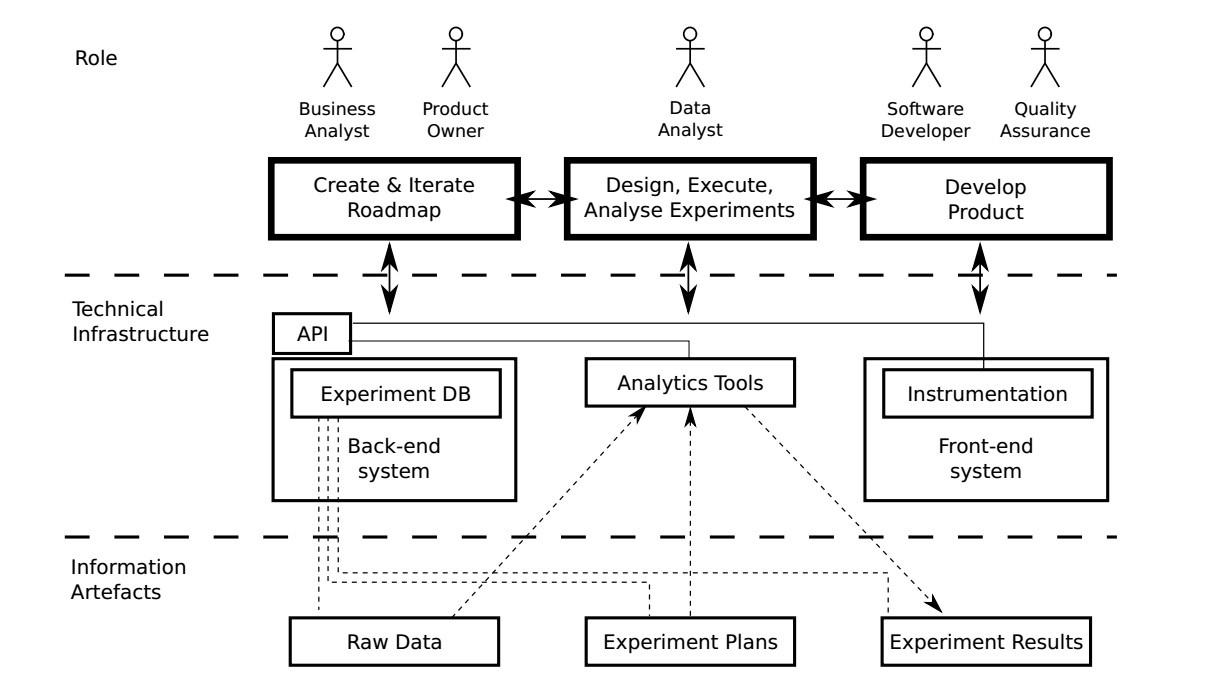
\includegraphics[width=5.0in]{infra.jpg}
	\caption{Continuous experimentation infrastructure \cite{fagerholm2014building}.}
	\label{fig4}
\end{figure}

The primary components of the introduced infrastructure are experiment database, analytics tools and instrumentation. The database stores raw data collected from the instrumentation and information related to the experiments, such as the logic for conducting the experiments and the experiment results. The analytics tools are used to perform data analysis on raw data from the experiment database to produce results regarding the experiment. The instrumentation is a part of the delivered software used to gather data regarding pre-defined metrics.  

\subsubsection{Experimentation stages and scopes}
Fig. \ref{fig5} introduces different stages and scopes for experimentation. For each stage and scope combination, an example technique to collect product performance data is shown. As startups often start new products and older companies instead develop new features, experiments must be applied in the correct context. Bosch states that for a new product deployment, putting a minimal viable product as rapidly as possible in the hands of customers is essential \cite{bosch2012building}. After the customers can use the product, it is often not yet monetizable but is still of value to the customer. Finally, the product is commercially deployed and collecting feedback is required to direct R\&D investments to most valuable features.
\begin{figure}[h]
	\centering
	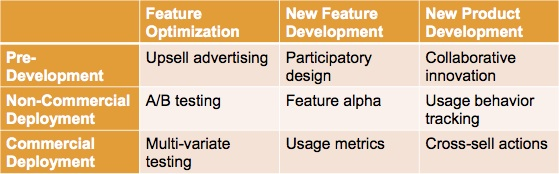
\includegraphics[width=5.0in]{scopes.jpg}
	\caption{Scopes for experimentation \cite{bosch2012building}.}
	\label{fig5}
\end{figure}

\subsubsection{Experimentation planning}
In continuous experimentation literature, the common way to plan experiments is to utilize the product strategy or roadmap \cite{ries2011lean, fagerholm2012building}. In the Lean Startup Build-Measure-Learn loop, the Learn phase is essentially a decision to whether to persevere or pivot the product strategy. However, this requires that the Measure phase is extensively planned in advance, so that a clear hypothesis exists. Essentially, the Build-Measure-Learn loop is very similar to the scientific Plan-Do-Study-Adjust loop. The single exception is that the Build-Measure-Learn loop is based on an assumption that the customer needs cannot be known even with planning. 

Fagerholm et al. emphasize the importance of analysing the data to test business hypotheses and assumptions, which have been created from the roadmap. These proven hypotheses can then be used to react to customers needs. The process for conducting experiments therefore starts from the business vision, then moves through planning and design phase to the technical implementation of the experimentation and data collection instrumentation.  

The first step required for a controlled experiment according to Kohavi et al. is to define an Overall Evaluation Criteria (OEC) \cite{kohavi2009online}. This criteria is the metric that the organization agrees to optimize with the experiment. Kohavi et al. cite Lewis Carroll saying "If you don’t know where you are going, any road will take you there". Attention has also to be paid to prevent running underpowered experiments, by determining the minimum sample size required for an experiment to be statistically significant \cite{kohavi2009controlled}.

\subsubsection{Data collection} 
To collect, aggregate and analyze the observations, raw data has to be recorded. According to Kohavi et al., some raw data could be for example page views, clicks, revenue, render time and customer-feedback selections \cite{kohavi2007practical}. The data should also be annotated to an identifier, so that conclusions can be made from it. Kohavi et al. present three different ways for collecting raw data. The first solution is to simply use an existing data collection tool, such as Webmetrics. However, most data collection systems aren't designed for statistical analyses, and the data might have to be manually extracted to an analysis environment. A different approach is local data collection, in which a website records data in a local database or log files. The problem with local data collection is that each additional source of data, such as the back-end, increases the complexity of the data recording infrastructure. The last model is a service-based collection, in which service calls to a logging service are placed in multiple places. This centralizes all observation data, and makes it easy to combine both back-end and front-end logging.

Feedback collection can be divided into two groups, active and passive feedback \cite{bosch2012building}. Active feedback includes collection methods where the customer is aware that he or she is providing feedback. Such collection tools are for example surveys. Passive feedback is collected while the customer is using the system, without the customer being aware of the collection. Examples of such data collection includes tracking the time a user spends using a feature, the frequency of feature selections, or the path through the product the user takes to perform a certain task. Bosch states that what makes the major difference between Innovation experiment systems and tradititional software systems is the low cost and ease of data collection in the former. 

An important aspect of collecting data is to pick the correct metrics. Metrics are numerical summaries used to compare variants of an experiment \cite{kohavi2009controlled}. Metrics range from simple aggregates, such as total page views, to complex measures such as customer satisfaction. One of the common pitfalls for experiments is to choose the wrong overall evaluation criteria \cite{crook2009seven}. This is especially important in the planning phase, where the wanted improved metrics are initially chosen. However, if the data collection layer is complicated, attention has to be paid that the metrics transition correctly from the planning phase to the implementation of the collection phase.  
\subsubsection{Data analysis}
To analyze the raw data, it must first be converted into metrics which can then be compared between the variants in a given experiment. An arbitrary amount of statistical tests can then be run on the data with analytics tools in order to determine statistical significance \cite{kohavi2009controlled}. 

In the analysis phase, attention has to be paid to other variables that might cause deviation of the OEC. As an example, Amazon showed a 1\% sales decrease for an additional 100msec of performance \cite{kohavi2007practical}. In certain cases time could cause deviations of the OEC and complicate experiment results. Kohavi et al. suggest conducting single-factor experiments for gaining insights and making incremential changes that can be decoupled. Another suggestion is to try very different designs, or in backend applications for example completely different algorithms. Data mining can then be used to isolate areas where the new algorithm is significantly better. Finally, using factorial design when factors are suspected to interact strongly is recommended. 

%"organisation needs a workfore to analyze qualitative + quantitative data"

\subsubsection{Roles in continuous experimentation}
Fagerholm et al. define five different roles in continuous experimentation: Business Analyst, Product Owner, Data Analyst, Software Developer and Quality Assurance \cite{fagerholm2014building}. The business analyst along with the product owner are responsible for creating and updating the strategic roadmap, which is the basis of the hypotheses. The basis for decisions are the existing experimental plans and results stored in a database. A data analyst is used to analyze the existing experiments and results and to create assumptions from the roadmap. The analyst is also responsible for the design and execution of experiments. The data analyst is in tight collaboration with the software developer and quality assurance, who are reponsible for the development of MVPs and MVFs. The software designers create the necessary instrumentations used to collect the data required by the analyst.

%question: what if there are no existing experimental plans, and this is the first experiment? how should the roadmap be created?
Another approach for the roles is introduced by Adams et al., who conducted a case study on the implementation of Adobe's Pipeline. Adobe's pipeline is process that is based on the continuous experimentation approach \cite{adams2013creating, adobe}. The innovation pipeline introduced in the study includes the following roles: designer, developer, researcher, product manager \cite{adobe}.

%http://www.janbosch.com/Jan_Bosch/Innovation_Experiment_Systems.html
\subsection{Continuous delivery and continuous experimentation collaboration}
As the experiments are run in a regular fashion, integrating experiments to the deployment pipeline should be considered. This requires changing the development process in such fashion that functionality is developed based on some actual data. The components required to support continuous experimentation include tools to assign users to treatment and control groups, tools for data logging and storing, and analytics tool for conducting statistical analyses.

TODO: finish
In the organization evolution path \cite{olsson2012climbing} continuous deployment is seen as a prerequisite for the experimental system. 
\subsection{Continuous experimentation in embedded software}
The purpose of analysing experimentation in embedded software in the context of this thesis is that B2B applications and embedded applications share similarities in the release cycle. The innovation ideas for embedded software are prioritized as a part of the yearly release cycle. This resembles the release model found in the case company, where some customers prefer to have new versions shipped every three months. By analyzing how experiments are implemented and the data collected in embedded software, information on how long and short release cycles differ can be gained. 

Eklund and Bosch have applied the innovation experiment system to embedded software \cite{eklund2012architecture}. In the study an embedded architecture for realising an innovation experiment system is presented. The study concentrates on what to evaluate in experiments in embedded software. The infrastucture for enabling the innovation experiment system is shown in \ref{fig6}.

\begin{figure}[h]
	\centering
	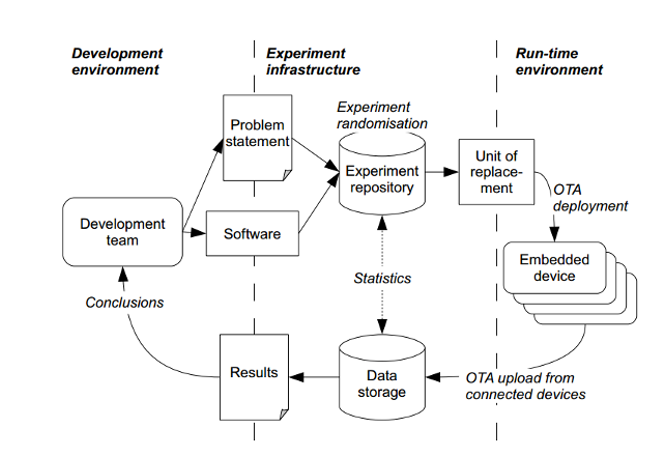
\includegraphics[width=5.0in]{embedded.png}
	\caption{Continuous experimentation architecture for embedded software \cite{eklund2012architecture}.}
	\label{fig6}
\end{figure}

The major difference between embedded and traditional software in terms of experimentation is the data collection phase. With embedded software, the data has to be either transferred over-the-air or on-board. With on-board measurements and analysis, the experiment manager autonomously controls when to run which experiments. 

%"Improvement occurs in individual software parts, but the underlying design concept remain mostly unchanged [3]"
%"The experiment infrastructure allows developers to deploy new software and collect data how it behaves in areal-world settings being used by actual users. The infrastructure support deployment of software experiments and collection of data over-the-air on a scale comparable to the entire customer base". 
%"The infrastructure supports with automated randomisation and factorial designs [6] sufficient to draw statistical conclusions from the experimental scenarios."
%"The experiment manager architecture, seen in Figure 3, supports the deployment of multiple experimental software parts to the same device and autonomously controls when to run which experiment, even allowing for local A/B-testing. Measurements and analysis is done on-board in real-time. The experiment scenario to be answered is implemented on the embedded device (i.e. how long does it take to . . . )"

The study also lists possible experiment scenarios supported by the architecture \cite{eklund2012architecture}. Possible experiment cases with the architecture are as follows:

\begin{itemize}
\item  How long does it take to . . 
\item  Which of . . . is most often used/accessed/. . .
\item  Identify behaviour that is not intended, e.g. menu selection followed by "back" indicates that the user made a mistake.
\item  Are there any features that are not used?
\item  Be able to evaluate competing designs based on the answers above, i.e. A/B testing (AKA. split testing).
\end{itemize}

%The initial focus of the innovation experiments would be
%on user interaction, but should be extended to other things,
%e.g. power consumption or precision in control systems. The
%experiments supported by the architecture could for example
%answer the following about real world usage, i.e. these are
%potential experiment response variables:
%• .
%• 
%• 
%• Are there any features that are not used?
%• 
\subsection{Challenges regarding continuous experimentation}
It is commonly found in the studies that the practiced experimentation is limited to optimizing narrow aspects of the front-end through A/B testing \cite{bosch2012building}. Additionally, experimentation is not often systematically applied \cite{bosch2012building}. Typically the imbalance between number of ideas that exist in the organization and the number of concepts that are tested with customers is enormous \cite{bosch2012building}. 

Some companies use traditional metrics such as the Net Promoter Score \cite{reichheld2003one} to gather feedback. These metrics however fail to guide the development process by providing timely feedback, and instead are backward looking and focusing on the whole product \cite{bosch2012building}.

One of the biggest challenges is also the architectural requirements set by the product to allow experimentation. According to Jan Bosch: "Collecting customer or performance data early in the innovation process requires changes to the R\&D processes, as customers need to be involved much earlier and deeper in the process. This also requires architectural changes of the product and platform to determine customer preference and interest." \cite{bosch2012building}.

%Jotain täältä?
%\cite{kohavi2012trustworthy}
%"Experimentation in practice is often limited to optimizing narrow aspecs of the front-end through A/B testing, and is not systematically applied" \cite{bosch2012building} 
%"Innovation in large organization is often characterized by an enormous imbalance between the number of ideas that, informally or formally, exist in the organization and the number of concepts that are in fact tested with customers." \cite{bosch2012building}
%"Traditional metrics such as the Net Promoter Score[Reichheld, F.F.: The One Number You Need to Grow] have been used for the last decade or more, but often fail to provide timely feedback during the development process as these are backward looking and focus on the entire product." \cite{bosch2012building}
%possible challenges in Lean startup: \cite{may2012applying}
%-Randomization algorithm and assignment method, data collection, storage, analysis \cite{kohavi2007practical}
Crook et al. investigate the common pitfalls encountered when running controlled experiments on the web \cite{crook2009seven}, which are listed in Table II. The Overall Evaluation Criteria (OEC) used in the first pitfall is a quantitative measure of the experiments objective. In experimental design, Control is a term used for the existing feature or a process, while a Treatment is used to describe a modified feature or a process. As a motivator for the first pitfall, Crook et al. introduce an experiment where the OEC was set to the time spent on a page which contains articles. The OEC increased in the experiment implementation, satisfying the objective. However, it was soon realized that the longer time spent on a page might have been caused by confusion of the users, as a newly introduced widget was used less often than a previous version of it. Aside from picking a correct OEC, common pitfalls deal with the correct use of statistical analysis, robot users such as search engine crawlers, and the importance of audits and control.
\begin{center}
\begin{table}[htb]
    \begin{tabular}{ | p{2cm} | p{10cm} |}
    \hline
	Pitfall 1 & Picking an OEC for which it is easy to beat the control by doing something clearly “wrong” from a business perspective \\ \hline
	Pitfall 2 & Incorrectly computing confidence intervals for percent change and for OECs that involve a nonlinear combination of metrics \\ \hline
	Pitfall 3 & Using standard statistical formulas for computations of variance and power \\ \hline
	Pitfall 4 & Combining metrics over periods where the proportions assigned to Control and Treatment vary, or over subpopulations sampled at different rates \\ \hline
	Pitfall 5 & Neglecting to filter robots \\ \hline
	Pitfall 6 & Failing to validate each step of the analysis pipeline and the OEC components \\ \hline
	Pitfall 7 & Forgetting to control for all differences, and assuming that humans can keep the variants in sync \\ \hline
    \end{tabular}
    \caption{Pitfalls to avoid when running controlled experiments on the web \cite{crook2009seven}.}
    \end{table}
\end{center}

\subsection{Motivation}
%However, based on the state-of-the practice section (describing 
%what is currently done in industry) you should motivate that the 
%problem you are addressing is a significant problem in industry 
%(you can include this justification at the end of the section).
%Why is this interesting?

The software industry is growing due to increasing digitalisation, and it is especially important for new and old companies alike to identify the problems relevant to customers and to stay flexible. Identifying the customers problems allows the companies purely focus on creating value, while staying flexible means quickly diverting development efforts towards currently desired features. The importance of continuous innovation is increasingly recognized in the literature \cite{steiber2013corporate}. Companies are also increasingly interested in utilizing real-time customer usage of the software to shorthen feedback loops \cite{olsson2012climbing}. 

The process of guiding product development with continuous experiments diminishes guesswork and instead provides a systematic approach. Avinash Kaushik states in his article Experimentation and Testing primer \cite{kaushik} that "80\% of the time you/we are wrong about what a customer wants". Mike Moran also found similar results in his book Do It Wrong Quickly, stating that Netflix considers 90\% of what they try to be wrong \cite{moran2007wrong}. A way to tackle this issue is to adopt a process of continuous experimentation. Ron Kohavi at Microsoft wrote "Features are built because teams believe they are useful, yet in many domains most ideas fail to improve key metrics" \cite{kohavi2013online}. Additionally, Regis Hadiaris from Quicken Loans wrote that "in the five years I've been running tests, I'm only about as correct in guessing the results as a major league baseball player is in hitting the ball. That's right - I've been doing this for 5 years, and I can only "guess" the outcome of a test about 33\% of the time!" \cite{moranmultivariate}.

%flexibility 
%no guesswork - systematic way
%"Companies are increasingly transitioning their traditional research and product development functions towards continuous experiment systems" \cite{olsson2012climbing}. 

\subsection{Existing case studies}
%At the end of the state-of-the-art section you should describe the differences
%between existing related research approaches (and especially existing 
%case studies) and compare them with your own goal in order to motivate your
%study.

%Previous works have presented case studies that exhibit di↵erent
%aspects concerning continuous experimentation. Steiber [23] report
%on a study of the model of continuous experimentation followedby Google, analysing a success story of this approach. Adams [1]
%present a case study on the implementation of Adobe’s Pipeline, a
%process that is based on the continuous experimentation approach.

Existing case studies regarding continuous experimentation have been conducted with varying aspects under concentration. Olsson et al. conducted a multiple-case study to explore companies moving towards continuous deployment and continuous experimentation \cite{olsson2012climbing}. In the transition phase from continuous integration stage to continuous deployment, the study investigates a telecommunications company with a highly distributed organization. The study considers transition from continuous delivery to continuous experimentation as a future research interest. 

Fagerholm et al. analytically derive a continuous experimentation model and apply it in practice in a startup company \cite{fagerholm2014building}. The study introduces an initial continuous experimentation model, examines the preconditions for setting up an experimental system and describes the building blocks required for such a system. The case company in this study is a relatively new startup company, and the company operates in the B2C domain. The study states that it is yet not clear how to determine the suitability of an experimental approach in specific situations. This is in line with the goal of this thesis: analyze the continuous experimentation approach in the B2B domain with two different software products.

Steiber et al. \cite{steiber2013corporate} have studied continuous innovation in Google. The study defines continuous innovation as "an experimental iterative process that operates successively to solve problems in markets characterized by turbulence, uncertainty and complex interactions". The study explores the organizational characteristics for continuous innovation in rapidly changing industries. The study finds that the entire organisation of Google is involved in continuous innovation. The study also states that there is a need for a more comprehensive analytical framework for continuous innovation, and also a need to study how to organize continuous innovation and continuous improvements.   

Adams et al. conducted a case study on the implementation of Adobe's Pipeline, a process that is based on the continuous experimentation approach \cite{adams2013creating, adobe}. The innovation pipeline introduced in the study consists of the following steps:
\begin{itemize}
\item Collect user problems
\item Identify problems worth solving
\item Prototype possible solutions
\item Live user testing + public releases
\item Refine, pivot or kill the idea
\item Build products that understand the user
\end{itemize}
The pipeline team consists of the following roles: designer, developer, researcher and product manager. The general principles found in the study are as follows:
\begin{itemize}
\item The idea will change
\item We're only right when the market tells us so
\item Create fast. improve constantly
\item Find the simplest thing that could possibly work
\item Define "success" before we build
\item Fail forward
\end{itemize}
The study is carried out in the company with over 10,000 employees. The study states that "there is a wealth of understanding about how small companies can innovate in a low-cost way in order to make small products viable". 

Kohavi et al. have widely studied online experimentation at microsoft \cite{kohavi2009online}. The experiments have been mostly performed in Microsoft's web sites with A/B testing, and the efforts have been proven succesful. This success further motivates the goal of this thesis of applying experiments in a different domain and different software products. However, as the study only consists of A/B testing, this thesis also inspects other kind of experiments performed in a continuous manner.
%Motivation: %Compare to my own goals
%  -clearly defined in the B2B context
%  -

\section{Case study as a research method}

\subsection{Case study}
Case study is a way to collect data through observation and to test theories in an unmodified setting \cite{zelkowitz1998experimental}. The case in a case study is the situation, individual, group or organization that the researchers are interested in \cite{robson2002real}. Kitchenham et al. found case studies important for industrial evaluation of software engineering methods and tools \cite{kitchenham1995case}. Runeson and Höst define it as a suitable research method for software engineering, since it studies contemporary phenomena in its natural context \cite{runeson2009guidelines}. It might not be possible to generate causal relationships from case studies as compared to controlled experiments. However, they provide a deeper understanding of the unit under study \cite{runeson2009guidelines}. An opposite type of research would be a formal experiment, with a narrow focus and control on variables. 

Case studies can serve different purposes. Robson defines four purposes as Exploratory, Descriptive, Explanatory and Improving \cite{robson2002real}. In an exploratory case study, the purpose is to seek new insights, find out what is happening and generate ideas and hypotheses for new research. Descriptive case study attempts to portray a situation or a phenomenom. Explanatory case study attempts to seek and explanation to a problem or situation, mostly in a causal relationship. An improving case study tries to improve an aspect of the studied phenomenom.  

%http://2012books.lardbucket.org/books/sociological-inquiry-principles-qualitative-and-quantitative-methods/s05-03-inductive-or-deductive-two-dif.html
Different approaches to the order of data collection, analysis and generalization can be categorized into inductive, deductive and abductive approaches \cite{dubois2002systematic}. In an inductive case study the research is conducted by first collecting the data, then looking for patterns and forming theorie that explain those patterns. Therefore an inductive approach moves from data to theory. A deductive approach, on the other hand, is in reversed order; the approach moves from general level to a more specific level. A deductive approach begins with studying what others have done, and then testing hypotheses that emerge from those teories. An abductive approach starts with the consideration of facts, or particular observations. These observations are then used to form hypotheses that relate them to a fact or a rule that accounts for them. The facts are therefore correlated into a more general description, that relates them to a wider context.

Runeson and Höst define the case study structure in five steps \cite{runeson2009guidelines}. First the case study is designed: objectives are defined and the study is planned. Then procedures and protocols for data collection are defined. Then the evidence is collected by executing the data collection on the studied case. The collected data is then analysed, and finally the results are reported.

Triangulation is a way to increase the reliability and validity of the findings. Triangulation means using different data collection methods or angles, and providing a wider picture of the case. Triangulation is especially important for qualitative data, but can also be used for quantitative data to compensate for measurement or modeling errors \cite{runeson2009guidelines}. Stake defines four ways to apply triangulation: Data triangulation, Observer triangulation, Methodological triangulation and Theory triangulation \cite{stake1995art}. In data triangulation, multiple data sources are used, or the data is collected at different occasions. In observer triangulation more than one observer is used in the study. In methodological triangulation different types of data collection methods are combined, such as qualitative and quantitative methods. In theory triangulation alternative theories or viewpoints are used.

Data collection in case studies tend to lean towards qualitative data that provides a richer and deeper view as compared to quantitative data \cite{runeson2009guidelines}. As a data collection method, semi-structured interviews are common in case studies \cite{runeson2009guidelines}. However, generalizing the results of a case study is often a subject of internal validity \cite{kitchenham2002preliminary}. It is especially important in a case study to address reliability and validity of the findings. Even with good faith and intention, biased and selective accounts can emerge \cite{robson2002real}. 

\subsection{Qualitative research}
Qualitative research attempts to answer to questions "Why?"" and "How?" instead of "What?", "Where?" and "When?" as compared to quantitative research. The most common way to collect qualitative data is via an interview. Seaman defines interviews as a way to collect historical data, opinions and impressions about something \cite{seaman1999qualitative}. The interview can be either structured, unstructured or semi-structured. In a structured interview the interviewer asks all of the questions, and the objectives are very specificed. The focus of a structured interview is to find relations between constructs, and the objective is descriptive and explanatory \cite{runeson2009guidelines}. In an unstructured interview the topic is broadly defined, and questions are asked also by the interviewee. In an unstructured interview open-ended questions are typical, and unforeseen types of information can be gained. The focus of an unstructured interview is on how the interviewee qualitatively experience the phenomenom, and the objective is exploratory \cite{runeson2009guidelines}. A semi-structure interview is a mixture of both open-ended and specific questions. Semi-structured interviews focus on how individuals qualitatively and quantitatively experience a phenomenom, and the objective is both descriptive and explanatory \cite{runeson2009guidelines}.

Seaman has explored qualitative research in software engineering context, and he defines different ways to analyse qualitative data \cite{seaman1999qualitative}. A typical way of analyziz is coding, which means extracting values for quantitative variables from qualitative data. Coding can also be used to organize the data based on themes and views. Seaman states that qualitative data is a lot richer than quantitative data, and using qualitative methods increases amount of information, diversity of information and confidence in results. 

%-Coding subjective data, select reference points for views, evaluate relability
%-Generation of Theory (GoT), extract from a set of field notes a statement or proposition supported in multiple ways by the data - – for use as hypotheses
%-GoT cross-case analysis: data divided into “cases”: two groups based on some attribute and examine similarities and differences (devs / management?) 
%-Confirmation of Theory: target: building up “weight of evidence"; triangulation; anomalies in the data
%-qualitative data is richer than quantitative data. use of qualitative methods increases
%– amount of information
%– diversity of information
%– confidence in results
The basic objective of data analysis is to form conclusions and theories from the data based on a chain of evidence. Qualitative data analysis can be divided into two different parts, hypothesis generating techniques and hypothesis confirmation techniques \cite{runeson2009guidelines}. Both of these techniques can be exploratory and explanatory case studies \cite{runeson2009guidelines}. In hypothesis generating techniques, a statement or proposition is extracted from the field notes that is supported in multiple ways by the data, and then used as a hypotheses \cite{seaman1999qualitative}. The data can also be divided into cases using cross-case analysis, where two groups based on some attribute are examined for similarities and differences. In the confirmation of theory, weight of evidence is built using triangulation of different data sources. 

%Quasi-statistical approaches, Template approaches, Editing approaches, Immersion approaches 
Robson introduces common features of qualitative data analysis in a sequential list \cite{robson2002real}. The first step is to code the initial set of data. Then, comments and reflections (referred to as 'memos') are added. After this the data is processed, similar phrases, patterns, themes, relationships and differences between sub-groups are identified. These identified patterns are then used to focus the next data collection phase. Gradually a set of generalizations are formed, that cover the consistencies discerned in the data. These generalizations are then linked to a formalized body of knowledge in the form of constructs or theories. 

In the sequential list, hypotheses are identified after the data has been coded. The hypotheses are then used to guide the following data collection process in an iterative approach. During the iterations, some generalizations can be formed, which eventually form a formalized body of knowledge as a final result.

Hypothesis generating techniques are for example "constant comparison method" and "cross-case analysis" \cite{seaman1999qualitative}. In the constant-comparison method the field notes are coded, text pieces are grouped into patterns and propositions that are strongly supported by the data are made. The propositions are then validated against any new data. In the cross-case analysis method data is divided into cases, such as two groups based on the same attribute. Pairs of cases are then compared to determine validations and similarities. 

The data analysis can be conducted with multiple different approaches, with each having a varying degree of formalism. Robson lists four such approaches, from least formal to most formal: Immersion approaches, Editing approaches, Template approaches and Quasi-statistical approaches \cite{robson2002real}. Immersion approaches are the least format, relying mostly on the interpretive skills of the researcher and having a low level of structure. Editing approaches include the usage of some codes which the researcher decides based on findings during the analysis. Template approaches, also known as template analysis, use priori codes to develop a coding template, organising the data based on themes. Quasi-statistical approach is the most formal approach, including quantitative calculations, such as word frequencies. Runeson and Höst state that editing approaches and template approaches are most suitable for software engineering case studies, as a clear chain of evidence is hard to obtain in immersion approaches, and word frequencies are hard to interpret \cite{runeson2009guidelines}. 

\subsubsection{Template analysis}
%http://www.hud.ac.uk/hhs/research/template-analysis/what-is-template-analysis/ 
Template analysis doesn't describe a clearly defined method, but rather refers to a related group of techniques used to thematically organise and analyse textual data \cite{king2004using}. Template analysis is a relatively structured process to analyse textual data, and has mostly been used to analyse data from individual interviews \cite{king2012doing}. The key component in template analysis is the generation of a coding template, which is initially formed on the basis of a subset of the data and then applied to further data. 

King defines code as a label attached to a section of text to index it as a relating to a theme or issue in the data \cite{king2004using}. As an example, codes can be defined to identify points in the text where an interviewee mentions particular categories of presenting problems. These kind of codes can be descriptive, and require no further analysis by the researcher. However, also codes requiring more interpretation can be defined. In template analysis, a key feature is to form a hierarchical organization of codes \cite{king2004using}. This way groups of similar codes are clustered together to form higher-order codes. This way the researcher can analyse the data at different levels of specifity, with higher-order codes giving a broad view and lower-order codes a more specific view. Parallel coding, where the same text segment is categorised with two different codes, is also allowed. 

The process of template analysis is to first create an initial template based on some pre-defined codes \cite{king2004using}. Then the template is revised by working through the data systematically while identifying and coding sections of interest in the text. Based on these findings, the initial template is modified, and finally develops to its final form. Modifications can be either insertion, deletion, changing scope or changing higher-order classification \cite{king2004using}. The final template is such that no sections of text related to research questions remains uncoded. 

The template is then used in interpretation to provide an account. King lists various guidelines that can be used in the interpretation of coded data \cite{king2004using}. The first guideline is to compile a list of all codes with some indication of frequency. The distribution of codes can then help to draw attention to the aspects of data with either multiple codes or missing codes. For example, if one interview in a set of interviews is missing a certain theme, analysis for possible reasons behind that missing code can be made. However, King suggests that while patterns can be used to draw attention to certain parts of the textual data, frequencies alone cannot be to gain any meaningful information. 

Another guideline is selectivity. King states that every code cannot be interpreted to equal degree of depth, and themes most relevant to understanding the phenomena under study must be identified. Prior assumptions of the researched shouldn't limit the analysis. Yet another guideline is openness, which King describes as taking themes judged as marginal into account. Themes that aren't of direct relevance to the initial research questions shouldn't be disregarded, as they can play a useful role in adding to the background of the study. Also themes lying outside the scope of the study should be included in the analysis, if they're considered to cast light on the interpretation of central themes in the study. Finally, King explains that purely linear relationships between codes, such as hierarchical relationships with subsidiary codes next to parent codes, "may not reflect the kinds of relationships a researcher may want to depict in his or her analysis". Instead, maps, matrices and other diagrams can be used to explore and display findings, and analysis doesn't have to stop when a full linear template is produced.

Finally, an account of the interpreted data has to be presented. As with interpretation, King provides three common approaches to presentation \cite{king2004using}. First of the approaches is a set of individual case studies, followed by discussion of differences and similarities between cases. This approach gives a lot of perspective of individuals, but can be confusing if the amount of participants is large. The second approach is an account structured around the main themes identified, drawing illustrative examples from each transcript as required. King states that this is the approach that most readily provides a clear thematic discussion, but the dangers is in drifting towards generalizations and losing sights of individual experiences. The third approach is a thematic presentation of the findings, using a different individual case-study to illustrate each of the main themes. The main problem here lies in selecting the cases which represent the themes in the data as a whole. King also adds that no matter which approach is used, direct quotes from participants is essential.  

\section{Research design}

Research design depicts the strategic decisions that guide how research is carried out \cite{denzin2000discipline}. This includes the studied phenomena, method selection, data-gathering and analysis. Different perspectives towards the researched subjects are usually categorized into two paradigms: positivist and constructivist \cite{gephart2004qualitative}. Positivism contents that an objective reality, which can be studied, captured and understood, exists. Postpositivism argues that reality can never be fully apprehended, but only approximated. Postpositivism therefore relies on multiple methods to capture as much of reality as possible. Constructivism assumes that multiple realities exist. A critical paradigm lies somewhere between positivism and constructivism, assuming that our ability to know of this reality is imperfect. To understand as much of reality as possible, it must be subject to wide critical examination. 

This thesis is based on the critical realist perspective. Critical realism studies people's perceptions to gain understanding of the reality that exists beyond these perceptions \cite{healy2000comprehensive}. Critical realism is especially suitable for case study research if the process involves thoughtful in depth research with the object of understanding why things are as they are \cite{easton2010critical}. 

During this research, the author was an employee at Steeri. Consequently, this case study is based on the participant-observer research method \cite{strauss1990basics}. Data triangulation is ensured by combining the observer results and interview results. 

%Triangulation is a way to increase the reliability and validity of the findings. Triangulation means using different data collection methods or angles, and providing a wider picture of the case. Triangulation is especially important for qualitative data, but can also be used for quantitative data to compensate for measurement or modeling errors \cite{runeson2009guidelines}. Stake defines four ways to apply triangulation: Data triangulation, Observer triangulation, Methodological triangulation and Theory triangulation \cite{stake1995art}. In data triangulation, multiple data sources are used, or the data is collected at different occasions. In observer triangulation more than one observer is used in the study. In methodological triangulation different types of data collection methods are combined, such as qualitative and quantitative methods. In theory triangulation alternative theories or viewpoints are used.

%the research underlying this case study is based on a participant-observer research method [1][3].
%Adler, P.A., Adler, P.: Observational Techniques. In: Denzin, N.K., Lincoln, Y. (eds.) Handbook of Qualitative Research, pp. 377–393. Sage, Thousand Oaks (1994)
%Corbin, J., Strauss, A.: Basics of qualitative research, 3rd edn. Sage, Thousand Oaks (2008)

The logical starting point of this thesis was the need by the case company to find a way to validate whether a feature is succesful or not. 

\subsection{Objective} %what to achieve?
%What does the company want to achieve
%What are the biggest problems
The purpose of this study is to seek ways to improve the product development process of two products within the case company, using practices known as continuous delivery and continuous experimentation. Existing documented implementations of continuous experimentation are primarily executed in the B2C domain, often with a SaaS product. Examples are the Microsoft EXP platform \cite{ep} and Etsy \cite{}. The focus of this study is in the B2B domain, with two applications that are not used as SaaS. 

\bigskip
\noindent \textbf{Research objective}
To analyze the software development process transition towards shorter feedback cycle and data-driven decisions from the perspective of the case company, with respect to continuous delivery and continuous experimentation practices.
%As the development process greatly varies in other teams inside the company, the focus is on a single team to narrow the scope.

The study is an exploratory deductive case study, which aims to explore how continuous delivery and continuous experimentation can be implemented in the case company. The study specifically aims to identify the main requirements, problems and key success factors with regards to these approaches in the context of the case company. Integrating these approaches to the development process requires a deep analysis of the current development process, seeking the current problems and strengths. Adopting both continuous delivery and continuous experimentaton also requires understanding the requirements of continuous delivery and continuous experimentation. To narrow the scope of the thesis, the focus of this thesis is in the development process of two different software products. The two different products were chosen so that cross-case analysis and therefore more generalizations can be made.

The research process starts by reviewing literature on both continuous delivery and continuous experimentation. In the literature review, main goals are to identify existing requirements and success factors in these approaches. Then interview is used to analyze and identify the pain points the company currently has in its development process. Then continuous delivery and continuous experimentation processes are viewed from the viewpoint of the case company, comparing the previously found benefits to the pain points in the case company's development process. As a result of viewing the practices from case company's viewpoint, necessary restrictions and requirements encountered in the B2B domain are obtained. Finally, the continuous experimentation infrastructure \cite{fagerholm2014building} is applied to the case company, and deviations listed. 

The research questions and research methods are summarize in Table 2.

\begin{center}
\begin{table}[htb]
    \begin{tabular}{ | p{3cm} | p{3cm} | p{3cm} | p{3cm} |}
    \hline
    \textbf{Knowledge gap} & \textbf{Research question} & \textbf{The focus of analysis} & \textbf{Data} \\ \hline
    B2B specific challenges in the practices & RQ 1: What are the B2B specific challenges of continuous delivery and continuous experimentation? & Empirical case supported by conceptual analysis & 13 interviews, documentations of the development process, literature \\ \hline
    Benefits of the practices after reviewing the challenges & RQ 2: How do continuous delivery and continuous experimentation benefit the case company? & Empirical case supported by conceptual analysis & 13 interviews, literature \\ \hline
    What deviations are there to existing models & RQ 3: How can continuous experimentation be systematically organised in the B2B domain & Conceptual analysis of continuous experimentation infrastructure by Fagerholm et al. \cite{fagerholm2014building}, and application of the model to case company. & 13 interviews, documentations of the development process, author observations \\ \hline
    \end{tabular}
    \caption{Research questions and research methods.}
    \end{table}
\end{center}

In this thesis along with confirming existing theories we do aim to generate new concepts and theories. The theory and case analysis are continuously matched to gain insights coherent with both theory and empirical observations. 

\subsection{Case descriptions} %what is studied?
%Be sure to specify as much of the industrial context as possible. In particular,
%clearly define the entities, attributes, and measures that are capturing the contextual information.

Experimental context needs the three elements: background information, discussion of research hypotheses, and information about related research \cite{kitchenham2002preliminary}. The two former will be discussed here, and the latter is introduced in the second and third chapters.

%-configuration management: no employer designed and no formal education

The company in question is Steeri Oy, which is a medium-sized company specializing in managing, analyzing and improving the usage of customer data. In this research, the units under the study are two teams responsible for developing two different software products. The first team is CDM, which is focusing on the respectively named software application. The other team is Dialog, also working for a respectively named software application. Both of the teams are managed by a similar structure, consisfting a team leader and a product owner, quality assurance and commercialization experts. 

The organisation of Steeri Oy is of a divisional type, with each business area forming independent teams based on the products and projects. The business areas of the whole company range from IT consulting to CRM implementations and development of own software products. To scope down the thesis, only teams doing development of own software products are in the scope of this thesis.
%The subteams of the first team under study have a common team leader, but different product owners and middle management. 
% describe organisation structure? %: https://docs.google.com/a/steeri.fi/spreadsheet/ccc?key=0Ai02aScOCplAdG9zQURicnlkM0ptTXhqbHN5ZE04X0E&usp=drive_web#gid=0

The unit of analysis is the development process of the two teams. The whole development process consists of the development framework used, but also of the interaction with customers, tools used in the current development process and the roles of individuals in the teams. The unit of analysis is studied by focusing on interviewing individual members at different positions in the organisation. The purpose of the interview is to identify the pain points in the current development process, which are then viewed against the benefits of continuous delivery and continuous experimentation found from existing literature. Analysis of implementing continuous delivery and continuous experimentation is then done based on the interview results.  

%Continuous deployment and continuous experimentation haven't been previously used by the case company. 
%In the beginning of the study, feedback was only collected in the form of bug reports from the customers. The bugs were then prioritized according to the importance, and added into the Trello workflow. 
%Under analysis is also the company's ways to interact with the customer.

The development process of the team is elaborated in detail in the chapter "State of the practice". In the following sections the general characteristicts of company, the two products and applied development processes are identified. The general charasteristics of the two teams under scope are then compared. The general characteristics are as follows. 

\begin{multicols}{2}
\begin{itemize}
  \item Product description
  \item Product environment
  \item Product architecture
  \item Usage
  \item Team composition
  \item Development practice
  \item Business model
  \item Programming languages
  \item Development tools
  \item Version releasing
  \item Unit testing
  \item Acceptance testing
  \item Feedback collection
  \item Usage data collection
  \item Feedback and usage data usage
\end{itemize}
\end{multicols}

The first three characteristics give us information on how the teams develop their software products. Usage then defines how and by whom the product is used in practice. The team composition and development practice provide important information on how the teams are composed and how they operate. Business model clarifies how the product is marketed, and how the product development is navigated in order to maximize revenue. Programming languages and development tools provide insight on the technical aspect of the development. Version releasing, unit testing and acceptance testing are taken into consideration when analyzing the transition towards continuous delivery, which eventually will automatize these phases. Feedback collection, usage data collection and data usage are analyzed to provide basis for the current feedback process operated by the case company, in order to gain insight on restrictions for continuous experimentation. 

\subsubsection{Dialog}
The Dialog subteam focuses on developing a multi-channel online marketing automation, iSteer Dialog. It is a software product designed to allow effective marketing on multiple channels, such as e-mail and websites, and to automate repetitive tasks. The product can be integrated to existing CRM solutions, and the data stored in CRM can then be effectively used for marketing purposes. 

\begin{description}
  \item[Product description.] Dialog is a multi-channel online marketing automation tool. The purpose of the product is to allow effective marketing on channels such as e-mail and websites, and to automate repetitive tasks. The product can be integrated to existing CRM solutions, and the data stored in the CRM can then be effectively used for marketing purposes. The product is primarily used through a comprehensive user interface by marketing professionals of customer companies. 
  \item[Product environment.] The product can be run on either servers provided by the case company or on the customers internal servers. Most of the customers use the product on the case companys own servers. Each customer using a provided server has an individual server and configurations, due to different integrations to the customers own systems. Customers running the product on their own servers form a minority.
  \item[Product architecture.] The product consists of a single maven-packaged project. Along with the actual product, several additional third-party or custom components are required. Such components are for example Typo3, which is an open source web content management framework, and a custom component used for SMS integration. Most of the components reside in the version control system, and the main product additionally resides in the CI system. Custom integrations to customers data sources, often based on a third party ESB tool, are individual components as well.
  \item[Usage.] Dialog is used by marketing professionals to automatize repetitive tasks. The user amount varies, but it is generally less than five human users per customer company.
  \item[Team composition.] The team consists of 3 software developers, a manager for commercialization, a product owner and a quality assurance engineer. The software developers don't have designated roles, and each developer is involved in every aspect of the product development process.
  \item[Development practice.] Development is based around a prioritized kanban board. Features are split into tasks by the product owner or team leader, and inserted into the kanban board. The developers then pick a single task from the sprint backlog column, complete it, and move it to the review column. From there the task undergoes quality assurance and delivery to the customer environment. The detailed development practice is introduced later in this chapter. The team is in the state of continuous integration, but the quality of automated tests isn't yet at the required level to lay confidence in builds working. 
  \item[Business model.] The product is still in the development phase, and is not sold as a ready package. The productization process is however ongoing, and the ideal situation is that the product can be sold as a ready package with only minor configurations per customer. The product is currently sold as a custom project, and requires installment to the customer environment and integration to the customers systems. The customer has also be trained to use the product, and after the product goes live the cooperation is continued with a support contract.
  \item[Programming languages.] The product is written mainly in Java, with the front-end built using JavaScript. 
  \item[Development tools.] The team uses GitHub as the version control system, and Jenkins as the integration server. Trello is used as the kanban board to manage projects, and Bugzilla is used as the bugtracker. 
  \item[Version releasing.] A new version is released when a customer requires a certain feature, and that feature has been completed. Updates for other customers are then released every two to three months on average. The release cycle length for customers in the development phase ranges from 2 to 4 weeks. 
  \item[Unit testing.] Unit testing is done by the developers whenever a feature is written. 
  \item[Acceptance testing.] Acceptance testing is performed by the product owner and quality assurance engineer of the team whenever a version is deployed to the customer environment. 
  \item[Feedback collection.] During development, acceptance testing is the main source of feedback. Some of the features are also developed for pilot customers. Feedback is also collected from customers in retrospective meetings after the projects, and received directly from customers via e-mail and meetings. Feedback isn't automatically collected in any way. The team has plans for in-product surveys and usage data analysis.
  \item[Usage data collection.] Usage data isn't collected at all.
  \item[Feedback and usage data usage.] The received feedback is discussed within the team to improve the development process or certain parts of the product. The feedback isn't systematically used,. 
\end{description}
%-java, javascript front?
%-frontend
%-binaries are built
%-jenkins deployed
%-which env decides
%-testing (written by coder, tested by uat?)
%-management

The software is configured and integrated to the customer environment as project work. This deployment doesn't require additional code as per customer, but only different configuration files. 

\subsubsection{CDM} 
The CDM subteam focuses on building a Master Data Management \cite{loshin2010master} solution, which integrates multiple customers data sources such as CRM, ERP and billing system to create a single point of reference. 

\begin{description}
  \item[Product description.] CDM is a Master Data Management \cite{loshin2010master} solution, which is used to integrate multiple customer data sources to create a simple point of reference. These data sources can include for example CRM, ERP and a billing system. The product also manages the data by removing duplicate records, matching same records and cleaning and validating the data with the help of external data such as the resident registration database. The product has an user interface that can be used for testing, but the product is primarily a background application without users. 
  \item[Product environment.] The product is installed to a customer environment, and certain custom specific configurations and rules have to be implemented for each customer. Such configurations are for example the integrations to customers systems and external identification services used. 
  \item[Product architecture.] The product consists of several maven-packaged projects, which in the build stage are added as a dependency under a single main project. The whole product can thus be packaged into a single web archive file.
  \item[Usage.] CDM is an integrated application, which is primarily only used by other applications. Therefore humans are only using CDM for debugging purposes.
  \item[Team composition.] The team consists of 4 software developers and a team leader. The software developers don't have designated roles, and each developer is involved in every aspect of the product development process.
  \item[Development practice.] Development is based around a prioritized kanban board. Features are split into tasks by the product owner or team leader, and inserted into the kanban board. The developers then pick a single task from the sprint backlog column, complete it, and move it to the review column. From there the task undergoes quality assurance and delivery to the customer environment. The detailed development practice is introduced later in this chapter. The team is in the state of continuous integration, but the quality of automated tests isn't yet at the required level to lay confidence in builds working. 
  \item[Business model.] The nature of the product requires customer integrations to customers systems, which are currently mostly done as manual work. In the ideal situation the product contains automated integration, and could be sold as a ready product with minor configuration work. Currently the product is sold as a custom project, and requires installment to the customer environment and integration to the customers systems. After the product goes live the cooperation is continued with a support contract.
  \item[Programming languages.] The product is written in Java.
  \item[Development tools.] The team uses GitHub as the version control system, and Jenkins as the integration server. Trello is used as the kanban board to manage projects. 
  \item[Version releasing.] A new version is released when a customer requires a certain feature, and that feature has been completed. Updates for other customers are then released every two to three months on average. The release cycle length for customers in the development phase ranges from 2 to 4 weeks. 
  \item[Unit testing.] Unit tests are required for new features, and are written by the developers during of after the feature implementation.
  \item[Acceptance testing.] Acceptance testing is performed by either a developer or the team leader whenever the version is deployed to a customer environment.
  \item[Feedback collection.] During development, acceptance testing is the main source of feedback. Feedback is also collected from customers in retrospective meetings after the projects, and received directly from customers via e-mail and meetings. Feedback isn't automatically collected in any way.
  \item[Usage data collection.] Usage data isn't collected at all.
  \item[Feedback and usage data usage.] The received feedback is discussed within the team to improve the development process or certain parts of the product. The feedback isn't systematically used,. 
\end{description}

\subsection{Context} %frame of reference

The previous chapter introduced the two teams and products under the scope of this thesis. The more general context of the whole company under study is defined by the following properties. 

\begin{description}
  \item[Company size.] Steeri has approximately 80 employees at the writing of this thesis. The employees are located in two cities in Finland, and many of the employees are assigned to projects at other organizations.
  \item[Business area.] The company in question focuses in managing, analysing and improving the usage of customer data. This includes various CRM-systems, such as Oracle Siebel, but the company also has its own marketing automation and master data management products. The company also does data analytics within the Business Intelligence team.
  \item[Teams under study.] As Steeri covers a wide business area, the scope for the thesis is narrowed down to two teams. The other team focuses on product development of a marketing automation product, while the other focuses on a master data management product. Both of the teams consist of developers, managers and Q\&A dealing with the same products.
  \item[Team setup.] The development team consists of a team leader and developers, while the management team consists of two product owners, commersialization manager and a requirement engineer. 
  \item[Development practices.] Currently the team in question uses continuous integration, with feature branches merged into mainline as soon as the feature is finished. This could differentiate from a couple of hours up to multiple days.
  \item[Development model.] The development model is essentially a Lean model, the core being a prioritized Kanban board.  
  \item[Tools used.] The teams under study use Git as a version control system and GitHub code review tool, Trello as the Kanban board for task management, Jenkins as the continuous integration server and Bugzilla for issue tracking. Various other tools, such as the hour logging system, CRM system and various other ticket logging tools exist as well.  
\end{description}

\subsubsection{Development process}
The development process of the case company has evolved from traditional, waterfall-style development through an agile phase to the current Lean approach based on a kanban board. In the very first phases, when the company was young, tasks were simply put into excel. Eventually, Agilefant backlog product management tool was introduced and tasks were moved into it. Scrum and agile practices were also adapted at the same time. Agilefant allowed sprint management, but caused too much overhead according to the developers. However, during the time Agilefant was used as the product and sprint backlogs, a part of Dialog development was offshored. Agilefant allowed easy tracking and managing the offshore development efforts.

After Agilefant was determined to cause too much overhead, Scrum whiteboard was used for a while. The physical whiteboard however caused issues with offshore participants. After the Development and Integration team was split further into two sub-teams focusing on each project, Scrum meetings were also seen as overhead. This was caused by only half of the team being interested and attached to tasks considering a single product. After it was decided that the team is split into two sub-teams, practicing Scrum was again seen as an overhead due to the low amount of participants. Eventually the whiteboard was replaced with an online kanban board, Trello. By the same time the Scrum meetings were abandoned for a more streamlined process, that is able to respond to changing requirements faster. 

Work items are first added to customer backlogs in iSteer Contact. In this phase they might be just initial skeletons and do not need to contain all needed information. The work items are added by product or business owners or project managers. At this phase the created backlog items are not yet visible in team backlogs in iSteer Contact. The idea is to list them in the customer backlog as early as possible and start refining the requirements collaboratively both offline and online with the help of tools such as Chatter. Chatter can be used to discuss a single story or the complete backlog.

When the backlog item is ready for the development team to start working on it, it should contain at least the following information:
\begin{itemize}
\item  A descriptive name
\item  Specifications that explain both the technical side and the business side
\item  Agilefant link four hour reporting
\end{itemize}
%The backlog item is added to team backlog by selecting the “show in team backlog” -option.

Team backlog is a view to all stories assigned to one selected team. It is a tool to collect and organize stories from all customer/project backlogs without cloning details into multiple places. It is a view of all “in team backlog” stories that are not yet completed and are assigned to the selected team. Team backlog items are prioritized and estimated once a week, and new stories will be moved to Trello when accepted by the development team. Stories can be moved to Trello by project managers or product owners, but they must be checked by team leaders who then move them forward into the sprint backlog or prioritized list columns.

\begin{description}
\item[Overview.] Trello is a project management application that uses Kanban to control the production chain from development to release. Kanban attempts to limit the work currently in progress by establishing an upper limit of tasks in the backlog, thus avoiding overloading of the team. Trello consists of multiple boards, each representing a project or a development team. A board consists of a list of columns, and each column consists of cards. Columns each contain a list of tasks, and cards progress from one column to the next when each task has been completed. A card is essentially a task, which is added by the Backlog Owner, and can be checked out by a developer. In Steeri, the columns used are Sprint Backlog, In Progress, Review, Ready, Verified and Done. 
\item[Sprint backlog.] The Backlog Owner moves the cards that have the highest priority into the sprint backlog. The sprint backlog should always contain enough cards so that whenever a developer completes a task something new is available in the backlog.
\item[In progress.] The actual development work is done in this stage. The actor here is the developer. The checklist to move a card into review stage is:
\begin{itemize}
	\item  All tasks are complete
	\item  Changes are pushed to a feature-specific branch
	\item  Unit tests are written and pass in the CI server
	\item  Feature is well-written and does not need refactoring
	\item  Pull request is created and a link is added to the comment field
	\item  Feature has been documented as needed
\end{itemize}
If the feature needs refactoring a task list must be created and the card moved back to In Progress column.
\item[Review.] Here other developers review the new code and deploy it to a development environment. Checklist for moving the card into ready stage is:
\begin{itemize}
	\item  Pull request is reviewed by at least two (2) persons
	\item  Pull request is merged to the development branch
	\item  Feature is deployed to a development environment
	\item  Source code quality has to be good enough!
\end{itemize}
After a developer has reviewed the pull request, he leaves himself as an assignee. The second person who reviews the pull request is responsible for cleaning all the assignees and moving the feature to Ready column. If there is a major problem in the pull request the feature should be moved back to Sprint Backlog and the yellow “Boomerang” tag added. Person who created the pull request is responsible for implementing the necessary remarks.
If only small fixes are needed, they should be implemented within the Github pull request workflow.
The second person who has reviewed and accepted the pull request is responsible for deploying the feature to a development environment.
\item[Ready.] Here the product owner verifies the new functionality in the development environment. The card can be moved to Verified if the feature has been verified by the Product Owner in the development environment. Product owner is responsible for moving the feature to the Verified column.
If verification for the feature fails, the Product Owner should move the feature back to Sprint Backlog column with the highest priority. In addition the Product Owner should add a yellow “Boomerang” label with a comment describing the results in the feature.
\item[Verified.] Here the backlog owner collects the timestamps and trello flow data. The timestamps depicts the duration it took from a card to process through the whole chain. The data is then used to analyze which columns the card spent the longest time in, and to identify the pain spots.
\item[Done.] This column simply states that the task has been completed, and should eventually be archived. There’s currently no general validation required from the customer, as the customer projects each have a different schedule and process for builds.
\item[Prioritized lists.] The backlog owner adds tasks to prioritized lists from team backlog as soon as the tasks meet the required criterias, contain the required information and are inspected by both the stakeholders and the backlog owner.
\end{description}

\subsection{Methods} %how to collect data? 
The primary source of information in this research are semi-structured interviews \cite{runeson2009guidelines} performed within the CDM and Dialog teams. The interview consists of pre-defined themes as follows: (1) current development process, (2) current deployment process, (3) current interaction with customers, (4) software product and (5) future ways with continuous delivery and continuous experimentation. Data is also collected through the product description documents and development process documents to verifying and supplementing the interview data. Data triangulation is implemented by interviewing multiple individuals. Methodological triangulation is implemented by collecting documentary data regarding the development process from internal documents. 

%miksi tutkimuskysymyksiin voidaan vastata haastattelututkimuksella?
The interview was chosen as a data collection method because of the nature of the research questions. Since the study focuses on applying two development methods to the development process of a team, individual perceptions of members are required. As the case study doesn't include a technical implementation, quantitative measurements to properly measure the effects before and after implementation isn't an option. The research questions cannot be properly supported with quantitative data. There is also a uncertainty about how much information the interviewees are able to provide, and thus the questions are mostly open-ended. The nature of interviewees opinions on the research questions are also not known in advance, and quantifying it isn't simple. 

%miksi haastattelukysymykset vastaavat tutkimuskysymyksiin?
In order to answer the research questions, information regarding the development process, customer interaction and feedback, deployment process and technical product details are required. The interview is divided into themes to address these aspects. The interview questions address, among other things, the specific situations and action sequences of the interviewee rather than general opinions. 

\subsubsection{Data collection} %TODO: Visualize two participated in the data collection
The interview is a semi-structured interview with a standardized set of open-ended questions, which allows deep exploration of studied objects \cite{runeson2009guidelines}. The interviews are performed once with every subject. Leading questions are avoided on purpose, and different probing techniques such as "What?"-questions are used. The interviews are performed in the native language of the interviewee if possible, otherwise in English, and are recorded in audio format. The audio files are then transcribed into text.

%miksi olen valinnut semi-structured interview:n
The interview begins with a set of background questions, used in coding the interview data per subject. After the introductory questions, the main interview questions make up most of the interview. The interview session is structured based on areas under study rather than based on a specific model. The interview roughly consists of five different areas: development process, deployment process, customer interaction, feedback and usage data, and experimentation.

The development process questions aim to identify the current ways of working, including variances between different roles. The questions also identify the perceived problems and strengths in the development process, which are then used in analysing the potential process for continuous experimentation. 

The deployment process is examined from multiple point of views. This includes the customer point and view, developer point of view and management point of view. Emphasis is based on B2B specific issues and practices, which are often caused by differences in the software environment as compared to B2C.  

The customer interaction section analyses customer involvement in the development and deployment process. The section identifies where the customer's presence is high, what is the role of the customer in the operational level and how the role of the customer affects the transition towards continuous delivery and continuous experimentation. 

Feedback and usage data collection section analyses the procedure of collecting and utilising the data. The section aims to identify the manners in which feedback is received, collected and systematically used. The section also analyses how different roles interact with the customer. 

The experimentation section analyses the possibilities of conducting experiments to guide the development process in the case company. This includes technical details, such as instrumenting the software components with data collection mechanisms and external usage data collection components, and storing the data in customer environment. The section also includes more specific questions, such as possible challenges faced in A/B testing and issues in quickly deploying experiments to the customer environment.  

%miksi valitsin nämä haastateltavat
Interview data is primarily sought from the developers of the development teams and the managers of the team. As the focus of the thesis is on the development process of two different teams, all participants of the team and its management team are interviewed. Process data is sought from the process documents made by the team. Quantitative data, such as the Trello ticket flow time, is sought from Trello. Data regarding the development process is also collected from the internal documents.

During the interviews, it was soon detected that the interviewees are able to give accurate answers to certain contexts based on their positions. This eventually contributed to the template analysis, where the data was better organised based on roles. Developers are most aware of the product and project context, including technical details and project details. Team leaders are mostly aware of the process and project context. They are the persons who are most able to explain the development process in detail. The team leaders are also most proficient in feedback collection. The management is most aware of the company context, including the status of the organization and available resources in the company. 

To summarize, interviews were chosen as the main data collection method based on three criteria. Firstly, the nature of the research questions required insight on the company settings and opinions of the employees. Secondly, quantitative data cannot be used to answer to the research questions, as first initial understanding of the phenomena has to be formed. Thirdly, the analysis is divided into themes based on the software products, and qualitative data provided by interviews can be readily analysed according to themes.

\subsubsection{Data analysis} %http://en.wikipedia.org/wiki/Thematic_analysis#Phases_of_Thematic_Analysis
In this case study the data analysis is based on template analysis, which is a way of thematically analysing qualitative data \cite{king1998template}. The initial template was first formed by exploring the qualitative data for three themes: development process, deployment of software and experimentation. Through multiple iterations of the data, multiple subthemes were then added to the three existing themes by further coding the data. Attention was paid to different roles of the interviewees.

Prior to the template analysis the data was inserted into a spreadsheet, where the rows represent codes of interest and columns represent interview subjects. This eased the analysis of data. The final template was formed after three iterations, which each increased the depth of the template by one or two levels, and the amount of codes by several.  

%minkä/miksi olen valinnut tietyn tavan analysoida ja koostaa vastauksista tulokset/johtopäätöksiä
Template analysis was chosen as an analysis approach because it makes it easy to organise and analyse the data according to themes. It is also particularly effective when comparing the perspectives of different participant groups \cite{king2004using}. Since the thesis focuses on multiple themes and the interview on multiple groups, template analysis was seen as a suitable approach.   

The results are formed from the final template, and structured according to themes of the research questions to answer the research questions as comphrehensive as possible. The results are then validated from the original interview data, so that none of the sections left out of the template are in conflict with the findings.

%The process of template analysis is to first create an initial template based on some pre-defined codes \cite{king2004using}. Then the template is revised by working through the data systematically while identifying and coding sections of interest in the text. Based on these findings, the initial template is modified, and finally develops to its final form. Modifications can be either insertion, deletion, changing scope or changing higher-order classification \cite{king2004using}. The final template is such that no sections of text related to research questions remains uncoded. 

%The template is then used in interpretation to provide an account. King lists various guidelines that can be used in the interpretation of coded data \cite{king2004using}. The first guideline is to compile a list of all codes with some indication of frequency. The distribution of codes can then help to draw attention to the aspects of data with either multiple codes or missing codes. For example, if one interview in a set of interviews is missing a certain theme, analysis for possible reasons behind that missing code can be made. However, King suggests that while patterns can be used to draw attention to certain parts of the textual data, frequencies alone cannot be to gain any meaningful information. 
% tabulation \cite{runeson2009guidelines}, where coded data is arranged into tables to get an overview of the data. The data is organized by 


%"One example of a useful technique for analysis is tabulation, where the coded data is arranged in tables, which makes it possible to get an overview of the data. The data can, for example be organized in a table where the rows represent codes of interest and the columns represent interview subjects." \cite{runeson2009guidelines} 

%-roles (devs, business, PO's)

%If developers and business people agree, the company is heading to right direction 

%\section{Development process of the case company}
%an overview of the entire process, then refining the parts that are relevant for the problems 
%Steeri is a mid-sized company of 80 employees, focusing in managing and improving customer data usage. This includes CRM systems, business intelligence solutions, customer dialog and data %integration. Steeri has created Customer data management (CDM) and Customer dialog (Dialog) products, which are developed by two different teams. 

%These two teams develop in an agile manner, but the continuous integration process \cite{fowler2006continuous} and short feedback cycles aren't achieved yet. 

%The development isn't at all distributed, and no external party affects the development process. 

%Sprinteistä jatkuvaan prosessimalliin on oikeastaan vaatimus.

\section{Findings}
% Identify the problems 
% Select the major problems in the case 
% Suggest solutions to these major problems 
% Recommend the best solution to be implemented 
% Detail how this solution should be implemented 
This section summarises key findings of the case study. It is structured according to the research questions, allowing the progress from a higher-level perspective to more detailed view. First, the identified challenges in continuous delivery and continuous experimentation are listed and explained. Then, the benefits of applying continuous delivery and continuous experimentation are analyzed based on the current state of the case company. Finally, a continuous experimentation infrastructure by Fagerholm et al. \cite{fagerholm2014building} is mapped to the case company context, and deviations identified.

%\subsection{Perceived problems}
%What kind of problems were found?

%====B2B vs B2C in general====
%
%B2B
%-There is little to no personal emotion involved in the purchasing decision.
%-Your most effective marketing message will focus on how your product or service saves them time, money and resources.

%B2C
%-When you are marketing to a consumer you want to focus on the benefits of the product.
%-Their decision is more emotional. Consumers are different in that they demand a variety of distribution channels for convenience, not so with the B2B market. 
%-Consumers don't want to work to understand your benefits, instead they will want you to clearly point out the benefits to them. 

%=============================


\subsection{Continuous delivery: B2B challenges}
%When to use CD: http://www.continuousagile.com/unblock/cd_costs_benefits.html
%You provide an online service: Web, SaaS, PaaS, online gaming, online big data, or mobile apps with Web service back ends. If you provide online services, you need to move to continuous delivery, or your competitors will race ahead of you.

Software development practices and product characteristics vary based on the domain and delivery model. Typical B2C applications are hosted as SaaS applications, and accessed by users via a web browser. In the B2B domain, applications installed to customer environments are very common. This section analyzes the problems faced with applications that are installed and operated in customer environments when transitioning towards continuous delivery.

The challenges regarding continuous delivery will be analyzed in three areas: technical, procedural and customer. Technical aspect includes the environmental challenges, configural challenges and other challenges related to the software product and its usage. Procedural aspect includes the challenges regarding the development process of software. Customer aspect consists of the customer interaction and customer commitment.

\subsubsection{Technical challenges}
The technical challenges for continuous delivery are derived from the interview. A part of the interview focused on the current deployment process and customer interaction of the case company, and this process is then compared to the continuous delivery practice from literature review.

\begin{center}
    \begin{tabular}{ | p{12cm} |}
    \hline
    \textbf{Specific problem} \\ \hline
    Downtime is more critical for certain customers \\ \hline
    Automated testing has to be built on top of a matured software product \\ \hline
    Acceptance testing is performed by both the company and the customers \\ \hline
    Software is often integrated to multiple third party applications \\ \hline
    Software is often accompanied by multiple external components \\ \hline
    There exists multiple different configurations due to having multiple customers with different specifications \\ \hline
    Transferring the software product to diverse customer-owned environments requires different deployment configurations \\ 
    \hline
    \end{tabular}
\end{center}

%Downtime
Downtime of the case company's products can be fatal. According to the Dialog product owner, downtime causes end-users being unable to perform their job. Downtime can also interrupt ongoing customer tasks, possibly losing critical data in the progress. With CDM, downtime can cause other integrated systems to shut down due to too many failing requests. Currently the deployment time for both projects is negotiated with the customer to prevent these cases, and the version deployments are done when the system can be closed for a short period of time. In the continuous delivery process the deployment pipeline has to be designed to address the issue of downtime.

%-testing costs could be pushed at least partially to users
The developers perceive automated testing and test environments to be the largest technical task. Since both of the case company's software products have been in development for a long time, building a viable test automation has many challenges with architectural decisions and available workload. Along with unit and integration tests, a critical step of the deployment process is the manual acceptance testing phase. The acceptance testing is performed in varying ways. For Dialog, some customers require to perform manual acceptance testing in a UAT environment before the product can be deployed into production. Other customers trust the developers to perform the acceptance testing, and the deployment to production can be negotiated without it necessarily requiring to pass the UAT phase. In CDM, all of the customers perform manual acceptance testing in the UAT environment. The technical implementation therefore should make it possible to continuously deploy versions to the UAT environment, and by the push of a button to the production environment. However, if the versions are deployed to UAT very often, customers might feel encumbered by the amount of UAT testing. The customers also have to be informed whenever a new version is available to the UAT environment.
%While this task can, depending on the project and current state of tests, take up most of the resources in transition to continuous delivery, in B2B context some of the testing costs can be pushed partially to customer projects. 
%Automate testing

%Third party application integration
Both of the case company's software products are integrated to various third party applications and APIs. As CDM is a component that integrates various data source together, changes to the APIs communicating with these applications must be planned and discussed in advance. Based on the interview results, automatically updating the integrations requires an unduly amount of work seeing the results. 

%External components
It is also common for B2B applications to have external components that have to be configured when the software is installed or the APIs to these components changed. Therefore the configurations for these external components either have to be manually updated or automated as well. In the case company, both Dialog and CDM are integrated to multiple external components. Currently upon version change these integrations are manually updated when necessary. In continuous delivery, changes that modify the API and therefore break these integrations might have to be manually updated.

%Different configuration per customer
Both of the case company's products are used in multiple different customer environments. This introduces a problem of managing different configurations per customer environment and software instance. Multiple possible solutions exist for the configurations, however, such as creating custom profiles per customer with different configuration for each profile. In the case company the challenge is how to automatically determine which customer profile should be used for each environment.

One of the main differences between B2B and B2C is the production environment. While a company focusing on B2C often owns the product environment, in B2B domain it is common to install the software on customers environment. Along with the varying customer specific configurations, there exists varying customer environment specific configurations. The customer owned environment introduces multiple challenges: accessing the environment, transferring the software product to the environment and integrating the software to other components within the environment. These challenges related to transferring the software include firewall configurations, required certifications and user rights. The customers also have to be informed on actions performed in their servers. For certain environments, a VPN connections is required. A VPN connection often has a user limit, which can prevent automatic version deployment.

%According to Jan Bosch, "In an IES environment, there is only one version: the currently deployed one. All other versions have been retired and play no role." \cite{bosch2012building}". 


%Database versioning
%database needs to be versioned

%Firewall configurations
%Required certifications
%Missing user rights
%VPN user limit
%Environment

%-automate testing
%Continuous delivery requires you to set up and administer automated testing. You will need to write automated tests, and you will need to automate the configuration of test environments. In our experience, automating testing takes more time and effort than any other aspect of a continuous delivery rollout.

%-testing costs could be pushed at least partially to users
%In an experimental product, you can push some of the costs of testing onto users. We'll talk about this option when we cover testing and product management.


%Tällä hetkellä tiimin resurssit eivät riitä sen toteutukseen. Asiakkaiden pitää ymmärtää mistä on kyse. Asiakkailta pitää saada tähän lupa / sopimus. Tällä hetkellä tekninen haaste eniten on tietokannan versiointi johon on olemassa ratkaisuja. Integraatioiden automaattinen päivittäminen vaatisi ehkä kohtuuttoman paljon resursseja suhteessa siihen mitä saavutetaan. Itse dialogin päivitysten automatisointi olisi tehtävissä helpoiten. Yleinen smoketestaus olisi tehtävissä, mutta vaatii että testit kirjoitetaan, pitäisi tehdä paljon, ja niitä pitäisi ylläpitää. Tällä hetkellä tähän ei ole resursseja.  Ei voida siirtää aina uutta versiota, koska pitää pystyä takaamaan isolla varmuudella että asiat toimivat. Käytännössä se että sovitaan asiakkaan kanssa että vaihdetaan versio, ja tällöin laukastausiin automaattinen tuotantoonsiirto, olisi toimiva ratkaisu. 


%External components have to be configured
%Useampi asia joka pitää laittaa käyttöön, OpenAM, DJ jne. Jos yksikin unohtuu laittaa käyntiin, jotkin tuotteen palvelut eivät toimi. (Ulkoiset komponentit)	SaaS-tuotteena herokussa ei ole ongelmaa. 

%Database versioning


%Different configurations per customer


%Firewall configuratiosn

%In the IT-departments, customers have to be informed on actions in their servers. There might be firewall configurations, required certifications and missing %rights. 
%Required certifications
%Missing rights
%VPN user limit
%siirto voi olla haaste, sillä ympäristöt ovat asiakkaiden hallussa. yhteyden saaminen esim. windows-koneille vaatii VPN:n, eikä se ole aina yksinkertaista. esimerkiksi VPN:n käyttäjälimitit asiakkaille voivat olla täynnä.

%Integrating the software to third-party components

%Downtime

  %IT-puolelle täytyy ehkä ilmoitella mitä tapahtuu, tai pyytää heitä tekemään asioita mihin meillä ei ole oikeuksia. Saattaa olla palomuurikonffeja joita pitää säätää, tai toimittaa meille jotain sertifikaatteja. 


%(CDM) -Downtime -ei ihmiskäyttäjiä, olisi ihan tehtävissä. UAT:kin on, jengi varaa resurssit testaamiseen, en tiedä onko kykyä tehdä kaksi versiota ja deployata ne tuotantoon. jos asiakkaan testaajien pitää kerran viikossa mennä UAT:hen testaamaan uutta versiota, söisi se niiltä paljon resursseja. Ei uusi versio kuitenkaan huono tilanne ole, ei heidän välttämättä tarvitsisi sitä testata. UAT on käytännössä pakollinen ennen tuotantoa, Sanomilla on sitä testattu ja se on CDM:n kanssa varsin haastavaa kun pitäisi tietää mitä tulisi eksakstisti takaisin. pitää pelata ulkositen palvelijoiden (VTJ) pelisäännöillä kun ei voida tietää mitä palautuu. yhdellä datasetillä testaaminen on vähän turhaa, kun yhden datasetin toimiminen ei kerro meille käytännössä mitään.	Ei tietoa teknisistä haasteista.

\subsubsection{Procedural challenges}
The procedural challenges are analyzed based on the development process documentations of the company and the interview, in which a section was dedicated to the current development process of the case company. 

\begin{center}
    \begin{tabular}{ | p{12cm} |}
    \hline
    \textbf{Specific problem} \\ \hline
    UAT environment is a requisite for production release \\ \hline
    The development process drifts towards small feature branches from long-lived feature branches \\ \hline
	Triggering the compilation and deployment of large, modular projects \\ \hline
	The software has to be deployed to multiple customers \\ \hline
	Versioning is affected by having different customer profiles of the product \\ \hline
	Responsibility moves towards developers \\ \hline
	Management and sales loses track of versions \\
    \hline
    \end{tabular}
\end{center}

%UAT
%-UAT is often the norm and is required before anything is moved to production
%-in B2B, continuous deployment straight to production is very risky
The basic deployment pipeline in the case company first includes a deploy to UAT server, which is then tested manually by either the team or the customer. Only after the UAT version has been validated to work properly, can the production version be released. Based on the interview results, continuous deployment to production is seen very risky due to the applications playing a major role in running the customers business, and continuous delivery with deployments to a staging environment is seen as very beneficial. Therefore the deployment procedure has to be designed to allow testing the software in a UAT environment, and making it possible to manually trigger the deployment to production.

Both of the case company's products are developed with a branching model, where feature branches are first thoroughly developed and then integrated to the master branch. Only the master branch is ever released to the customer. However, with continuous delivery the long-lived feature branches should be changed to short-lived and relatively small feature branches to enable faster deployment of the software. The benefit of smaller branches is that while there may still be bugs, they're introduced in a fewer number of commits, and entire large features don't need to be rollbacked. Smaller branches also enable faster feedback. While the small feature branches might be common for companies with a relatively new software products, companies that have been developing products for a long time might be more devoted to the practice of feature branches.
%If the components are sufficiently small, it is preferable to have a single build for the whole application—giving the fastest feedback of all. \cite{cdbook}

%Pull requests

The software applications in B2B often are large and modular applications, as is the case in the case company. CDM is a software component that is compiled from multiple projects. As the deployment process is currently manually triggered by first releasing a version, a suitable time can be chosen each time. With continuous delivery the deployment process is triggered automatically, and with a modular project each module has to be in the correct state in order to produce a coherent version. The point when a deployment is triggered has to be designed to maintain the integrity of the application.
\begin{aquote}{CDM Developer}
"Pull requests aren't always working as is, due to the nature of CDM. There are dependencies between projects, and occasionally merges are done without the will to deploy. However, if pull requests are to be deployed when merged, a better picture of this process is needed for the developers."
\end{aquote}
In the case company, merging a pull request is not a valid trigger of a deployment, since pull requests are project specific. Some features require changes to multiple projects, and all of the pull requests have to be merged for the feature to work as intended. However, a good CI tool will handle the dependency management \cite{cdbook}.

%Multiple customer environments
Both of the case company's products are used by multiple customers, each having their own environment. As the deployments are currently done manually, the customers receiving each deployment can be manually chosen.However, with a continuous delivery process whenever a feature or a new release is ready to be delivered, it can either be deployed to a single customer or to every customer. Attention has to be paid when configuring the workflow to allow deploying to an arbitrary customer. If only certain customers accept updates on a continuous basis, it has to be possible to prohibit deploying to every customer at once. This is the case especially in the early stages, where all of the customers projects aren't yet in the state of continuous delivery.

%Versioning
Multiple customer environments affects versioning of the software product. In the case company, each customer has a unique configuration of the product, with possibly different versions of certain components. According to Jan Bosch, in an IES environment only a single version exists: the currently deployed one. Other versions are retired and play no role \cite{bosch2012building}. However, with multiple environments, multiple different versions of the software are necessary at least in the early phase. Eventually the product may be developed in such manner that a single version is sufficient. The build script therefore has to be configured to consider the customer-specific components when compiling the builds for each customer.

%"A final aspect is the avoidance of versioning of software. Traditionally, for many companies, every customer would ultimately have a unique configuration of the product with different versions of components making up the system. This adds a whole new layer of complexity to the already costly process of deploying new versions. In an IES environment, there is only one version: the currently deployed one. All other versions have been retired and play no role." 

%Developer responsibility 
Continuous delivery also drifts response towards the developer, and the developers decide what is ready to be released. Currently in the case company the product owners and team leaders are responsible for negotiating the deployment date with the customer, and they also inform the developers that a new version is required. If the developer can single-handedly deploy a feature, the management can quickly lose track on the features available to customers. This also requires the developers to deeply understand the details of the version control system and automated testing. 

Due to increased developer responsibility and varying interval of version updates continuous delivery causes, a team leader express concern that the delivery process complicates tracking when deployments are performed, and when features are finished. This also concerns other parties working in the customer interface, such as sales. While this is a concern for version deployments to the UAT environment, especially if developers perform these deployments at will, can production releases still be negotiated with the customer. Neely and Stolt have also found similar results \cite{neely2013continuous}, which they solved by providing mechanisms by which the parties if need of knowledge regarding release times could track the work in real time.  

%Neely and Stolt found out that with a continuous flow, Sales and Marketing departments lost the track of when features are released \cite{neely2013continuous}. Continuous delivery requires the company as a whole to understand the continuous flow process. Neely and Stolt solved this challenge by providing mechanisms by which the parties in need of knowledge regarding release times could track the work in real time \cite{neely2013continuous}. 


%-should the product be always deployed to every customer?

%jos pull requestit haluttaisiin deployata automaattisesti, eivät pullrequestit ole aina täysin toimivia sellaisenaan. riippuvuuksia niidän välissä, ja toisinaan mergetään ilman että halutaan deployauksia. nykyään tämä tieto liikkuu kehittäjien päässä. pitäisi saada tarkempi kuva jos pullrequestin triggeröinti aiheuttaisi deployauksen. yksi haaste on se että asiakkaita ja ympäristöjä on paljon. miten määritetään mille asiakkaalle deployataan? ei ole järkeä viedä asiakkaille jotka eivät ole sitä toivoneet. täysin automaattisesti vaikea tehdä, ja ihmisen pitäisi päättää mihin versio deployataan. muutokset saattavat vaatia muiden komponenttien päivityksen, tietokanta jne. niiden koordinointi voi olla haaste. myös jos CDM on integroitu muiden asiakkaiden tuotteisiin saattaa rajapinta vaihtua. siirto voi olla haaste, sillä ympäristöt ovat asiakkaiden hallussa. yhteyden saaminen esim. windows-koneille vaatii VPN:n, eikä se ole aina yksinkertaista. esimerkiksi VPN:n käyttäjälimitit asiakkaille voivat olla täynnä.

%CD costs http://www.continuousagile.com/unblock/cd_costs_benefits.html

%Costs

%-developer training: social commitment and understaind of the version control system
%Continuous delivery also involves developer training costs. Developers need to understand the details of their version control system. They need a full social commitment to automated testing. They must take more responsibility for delivering release-ready code and features.

%-understanding how major changes can be inserted and hidden unless they're ready
%Incremental releases are complicated. Developers must figure out how to insert major changes invisibly, and hide them with switches until they are ready to be released. This staged migration adds some complexity that is not present if you just rip out the old stuff and then test the new stuff. However, you will gain confidence by seeing changes working in production systems before you "unveil" them to your users. This can more than compensate for the increased complexity
%It is faster. You unblock your team so that developers can work at full speed. They don't have to wait for a product manager, product owner, or marketing person to tell them that users, marketing and documentation are ready for a release. Instead, they release everything that is ready, and hide it from the general public. The PM or marketing person can come along later, see that the new feature works, and start the "unveil" process.
%It provides the correct incentives. The developer is responsible for the release, because he or she is the one who can fix it. A developer can be called back from Friday night beers to fix a problem. Therefore, developers have a compelling reason to make a good decision about what to release. They should not throw buggy code over the all to a QA person. They need to be forced to focus on quality by removing the QA training wheels. They will be motivated to build good tests, and good scripts for testing and deployment.

%Developer responsibility
%Developers gain a lot of power and a lot of responsibility from continuous delivery.
%Developers (programmers) will decide what is ready to release. This is a strong finding. We see it in all successful continuous delivery organizations. The developer of a feature decides when it is ready, and runs the scripts to put it into the production version.

%http://www.slideshare.net/wakaleo/continuous-deliverywithmaven CD with maven

%http://blogs.atlassian.com/2014/07/skeptics-guide-continuous-delivery-part-3-real-world-pipelines/ Pipeline

%en näe että sitä saataisiin ikinä toimimaan nykyisellä kokoonpanolla. cdm koostuu niin monesta projektista, että käytännössä en tiedä miten voisimme automatisoida se. riippuen mihin projektiin on tuulut muutoksia, pitää ne releaseta ja laittaa cdm:n pääprojektiin joka ottaa muuttuneet releaset mukaan. release-numerot vaihtelee per aliprojekti, voi olla joko pieni- tai iso releasemuutos ja sen mukaan kasvatetaan releasenumeroa. jos olisi vain yksi projekti niin voitaisiin se automatisoida. yhden projektin tekemisessä ei sinäänsä ole haasteita. monen projektin idea on tällä hetkellä aika huono, sillä kun buildaamme cdm:n, buildaamme aina pääprojektin. yksikään aliprojektia ei buildata koskaan, pl. käyttöliittymä. hyöty siitä että ne on itsenäisiä projekteja on aika nolla. nyt kaikissa aliprojekteissa omat versionumerot, joka on aika huono ratkaisu. jos kaikki aliprojektit olisi kiinnitetty samaan versionumeroon koko CDM:llä, voitaisiin vain päättää että nyt ollaan tehty tällaiset muutokset CDM:ään. mietitään että meillä on githubissa kamat, jos haluttaisiin autodeployaa tuotantoversio asiakkaille, saataisiinko esimerkiksi pääsy kaikkiin asiaksympäristöihin että voisimme automaattisesti siirtää eri releasen? voisiko kantamigraatiot automatisoitua? mitä jos tuotantodataa pitäisi päivittää, saataisiinko sitä päivitettyä, tuskin. 

%UAT

\subsubsection{Customer challenges}
The customer challenges are analyzed based on two sections of the interview: customer interaction and the deployment process. 

\begin{center}
    \begin{tabular}{ | p{12cm} |}
    \hline
    \textbf{Specific problem} \\ \hline
    Customers are trained to use a certain UI \\ \hline
    Customers are reluctant towards new versions \\ \hline
    Changelogs are especially important, since customers depend on the software \\ \hline
    Pilot customer is required for developing the continuous delivery process \\ \hline
	Production deployment schedule has to be negotiated with the customer \\ \hline
	Ongoing critical tasks by users cannot be interrupted with downtime \\ 
    \hline
    \end{tabular}
\end{center}

%Customers have been trained to use a certain version of the product
One of the main issues found in the deployment of software is that some customers are reluctant towards new releases. One of the reasons for this reluctancy is that new releases occasionally contain new bugs. In the case company, customers using Dialog have been trained to perform certain tasks with a certain user interface. The customer might perform these tasks daily, once every two weeks or even less frequently. If the UI changes often, the customers feel lost and initially take more time to perform the tasks.  
\begin{aquote}{Dialog product owner}
"The user interface should be easy to use. Now it's relatively hard to learn. If customers have just learned to perform a task, and we change the UI, the feedback is terrible."
\end{aquote}

%Customer reluctancy towards new versions
Some customers are very reluctant against constant modifications and continuous version updates, since version updates occasionally introduce new bugs and modifications alter the user experience. While the user experience could be improved in the long run, the customers might feel frustrated when they have to learn to work with the modifications. The interviewees have ideas on how the reluctancy can be reduced. If modifications were made more often, it would lead to smaller modifications and might reduce the customer reluctancy towards new versions. When customers become accustomed to the model of continuous version updates, the reluctant attitude might change. Customers also need to understand the concept of continuous delivery, and that the features are eventually implemented to address customer needs and to improve the user experience in the long term. 
\begin{aquote}{Dialog product owner}
"If something changes, communication with the customer is hard. The customers feel that even if the version included very good changes, if something visible changes it gets alot of negative feedback".
\end{aquote}
The customers are unaware of the problems related to deployment issues unless the deployment has errors. However, if the version contains many UI changes the customer might feel frustrated by being unable to perform certain actions in the old way: 
\begin{aquote}{Dialog product owner}
"Customers have been doing this for their living - they're getting old, they have their own working histories and they're in the working mode. These persons don't approve alterations in the software, and they're not ready for the constant changes."
\end{aquote}

Listing the changed features in changelog entries is especially important when releases are made more often. While the changes become smaller the faster versions are released, the customers become less aware of when the version will be updated and when features have changed. Currently the version deployments are negotiated with the customers, and necessary actions are taken to explain the changed features to the customers in meetings or in e-mails. When the deployments are made more often, discussions regarding version releases may be reduced or even ceased.  

%Pilot customer
A way to identify the best practices in continuous delivery is to develop the continuous delivery process with a pilot customer. Pilot customer is a company willing to help the company to quickly learn what works and what needs to be improved. The interviewees expressed a desire to first test the continuous delivery process with a single customer that is willing to receive updates in a continuous manner, since the engagement model inevitably differs from the current model. Therefore the company can train customer interaction with continuous delivery, find the actual reasons for version reluctancy, see how the change in deployment process affects customer interaction and even test if the UAT environment is necessary.

%Deployment time and downtime
%A customer might be doing a critical task
Customers might be using the software when a new version is deployed, and the deployment process shouldn't interfere with ongoing usage. Therefore the most viable solution is to initially deploy the versions to the UAT environment. To prevent downtime and obstructing the usage of the software, the production deployment date should be negotiated with the customer. Production deployment might cause downtime, and cannot be made during times when critical tasks are performed. The test environments can be continuously updated, and once the customer is satisfied with the software and feels a need for a new version, deployment to production can be triggered.  

In the case company, the production deployment date is often negotiated with and specified by the customer, while the product can be deployed to UAT at will. UAT is also used by the customer to validate the functionality of the software, since the customer has ordered the product to perform certain tasks and fill certain criterias. However, the customers don't validate the versions at the UAT environment unless they are informed that new versions are available, since the UAT is not used for any other purpose than testing. 

%-Asiakkailla asenneongelma

%(Case-firma esittää että halutaan pilottifirma jotta mallia voidaan kokeilla)

%-To train customer interaction with continuous delivery
%-To test if UAT is necessary
%-..

%\begin{aquote}{Dialog developer}
%"Customers need to understand what continuous delivery is all about."
%\end{aquote}



%Tällä hetkellä tiimin resurssit eivät riitä sen toteutukseen. Asiakkaiden pitää ymmärtää mistä on kyse. Asiakkailta pitää saada tähän lupa / sopimus.
%Jos kokoajan julkaistaan uutta versiota, uusi versio ei tunnu uudelta versiolta koska muutokset ovat niin pieniä. Tämä voisi vähentää muutosvastarintaa. Jotkut käyttäjät ovat muutosvastaisia, jotkut nauttivat siitä. 
%If we made the versions more often with smaller changes, this could reduce the rebellion against version updates. 

%Some customers don't want UI changes, since they have been trained to perform certain tasks with a given UI. The customer might use the product once every two weeks and then get confused if the UI varies. Therefore the UI should have a stable consistency. 
%-however, 

%Hyvä että he validoivat toiminnallisuuden. Downtimeä voi tulla, mutta siirrot ovat yleensä varattuja siihen aikaan kun ei ole asiakkaan työaika. Dialogia käyttää vain asiakkaan työntekijät suoraan, vain virka-aikaan eikä yöllä tai viikonloppuisin.     Ei ainakaan tavallisesti. Ei, pysyy poissa sen ajan. Jotkut halusivat itse testata sitä ja tehdä itse testicaseja. Heillä on testi- ja tuotantodialogit, muilla ei. Ei tarvitse.
%Asiakas validoi ohjelmiston toimivuuden.   Asiakkaalla on downtime silloin kun siirretään tuotantoon. Testaavat uutta versiota testiympäristössä.  Ei muutakuin korkeintaan haluamassa versiota. Sovitaan päivä. Ei muuten kuin päättää ajat. Tuotanto on kuitenkin alhaalla kun versio siirretään. 


%The deployment time has to be negotiated with the customer

%Käytännössä se että sovitaan asiakkaan kanssa että vaihdetaan versio, ja tällöin laukastausiin automaattinen tuotantoonsiirto, olisi toimiva ratkaisu. Jos kokoajan julkaistaan uutta versiota, uusi versio ei tunnu uudelta versiolta koska muutokset ovat niin pieniä. Tämä voisi vähentää muutosvastarintaa. Jotkut käyttäjät ovat muutosvastaisia, jotkut nauttivat siitä. 

%pitää katsoa asiakkaan kanssa milloin heille käy versionpäivitys. 	Kun deployataan, palvelin täytyy pysäyttää ja laittaa varapalvelin pystyyn. 

%A customer might be doing a critical task with the software component, and therefore automatic version changes shouldn't cause downtime. 
%Jos asiakkaalla on jokin Dialogin lähetysprosessi kesken, esim. Laakkoselta tulee paljon paljon päivittäin klo 10 tai 9 päivityksiä. Jos tehdään päivityksiä automaattiesti, mitä silloin tapahtuu? Jos YIT haluaa lähettää huomenna kello kymmeneltä sähköpostilähetyksen, mitä tapahtuisi?  Periaatteessa pitäisi aina tietää asiakkaan tarve. Eräs asiakas ei halua että UI muuttuu, sillä heillä tulee todella paljno käyttäjiä. Joku joka käyttää tuotetta kerran puolessa kuukaudessa ihmettelee, jos homma on yhtäkkiä erinäköinen. Pikkumuutokset varmasti palvelevat kaikkea. Asiakkaita saattaa ärsyttää, jos tuote muuttuu kokoajan liikaa. Se voidaan kokea epämukavaksi. Pitäisi olla perus pysyvyys, vaikka kuinka menisi parempaan suuntaan. 	Haaste olisi käyttäjien informoiminen. Käyttöliittymän pitäisi olla niin helppo. Nyt käyttöliittymä on vaikea, ja nytkin on vaikea osata käyttää, että kun he ovat juuri oppineet jonkin asian. Kun reaaliaikaisesti muutamme sitä yhtäkkiä, palaute on hirveätä. Jos se olisi helppoa, niin se ei olisi niin iso ongelma. Asenneongelma joka kuvattiin aiemmin. 

%(DIALOG)

%===============
%Delivery B2C:

%"Most customers of most products hate new releases. That's a perfectly reasonable reaction, given that most releases of most products are bad news. It's likely that the new release will contain new bugs. Even worse, the sad state of product development generally means that the new features are as likely to be ones that make the product worse, not better. So asking customers if they'd like to receive new releases more often usually leads to a consistent answer: No, thank you. On the other hand, you'll get a very different reaction if you ask customers next time you report an urgent bug, would you prefer to have it fixed immediately or to wait for a future arbitrary release milestone?" \cite{http://www.startuplessonslearned.com/2009/12/continuous-deployment-for-mission.html}

%Mindsets:

%"if a change is supposedly side effect free, release it immediately. "

%"The second shift in mindset required is to separate the concept of a marketing release from the concept of an engineering release. Just because a feature is built, tested, integrated and deployed doesn't mean that any customers should necessarily see it."

%"Plus, you want to get good at selectively hiding features from customers. That skill set is essential for gradual roll-outs and, most importantly, A/B split-testing. In traditional large batch deployment systems, split-testing a new feature seems like considerably more work than just throwing it over the wall. Continuous deployment changes that calculus, making split-tests nearly free. As a result, the amount of validated learning a continuous deployment team achieves per unit time is much higher. "


%Typical B2C applications are hosted as SaaS applications, and accessed by users via a web browser. In the B2B domain, applications installed to customer environments are more common. 
\subsection{Continuous experimentation: B2B challenges}
The case company's two software products differ on how they are used by the customers. In this section, continuous experimentation challenges are analyzed for general cases encountered in both products, and special cases encountered in a single product due to a specific product characteristic. 

The challenges regarding continuous experimentation are analyzed in four areas: technical, organizational, customer and A/B-testing. A/B testing was chosen as an examined subject of its own, since it is a commonly known experiment, and the difference between the case company's products affect especially A/B testing.  

Technical aspect includes the data collection, measurable metrics and other challenges related to the software product and its usage. The organizational aspect includes challenges related to the organizational culture, financing and ways of working. The customer aspect includes the challenges regarding the experiments in the customer interaction process and from customers point of view. A/B testing section analyses the viability of guiding the development process of both products with A/B tests.
\subsubsection{Technical challenges}
The technical challenges are analyzed based on both the product description documents and sections of the interview focusing on experimentation and feedback.

\begin{center}
    \begin{tabular}{ | p{12cm} |}
    \hline
    \textbf{Specific problem} \\ \hline
    Not having a UI limits the scope of experiments in CDM \\ \hline
    Low end-user volume limits experiments that rely on statistical significance \\ \hline 
	CDM is only usable via API calls, which limits the scope of experiments \\ \hline
	Measurable metrics for the software products are not extensively identified  \\ \hline
	Experimental architecture has to be implemented on top of a matured project \\ \hline
	Data has to be collected in customer environments \\ 
    \hline
    \end{tabular}
\end{center}

%No user interface
%Only used via API calls
The case company's products represent two different styles of software products. While Dialog is used by users via a UI, CDM is used by other systems via a REST API. As CDM is a software component which is primarily used by other systems via API's and certain calls, tracking user behavior doesn't provide as much input as with a user interface. CDM also isn't used by an user interface, which limits the possibilities for A/B testing. While it is possible to experiment with a software component that has a UI and human users by employing A/B testing, other experiments have to be conducted on software without direct user access. Such experiments include feature alpha, usage metrics, usage behavior tracking and participatory design, among others \cite{bosch2012building}.
%Statistical significance
%TODO: kerro tarkemmin mitä experimenttejä

%Low user amount
The lower user amount also affects the types of suitable experiments. Dialog has only approximately five users per customer, while CDM has no human users at all. Experiments relying on statistical significance, such as A/B testing and multi-variate testing, lose most of their value with a low user volume. To be able to confirm validations with such experiments require a varying amount of users depending on the conversion rate of the experiment. The company then either has to work with a lower confidence interval, or have a very high conversion rate to reduce the amount of subjects needed for statistical importance. However, many experiments rely on tracking and improving the usage behavior and not relying purely on statistics. A product owner views experiments relying on tracking the user actions suitable for developing Dialog:
\begin{aquote}{Dialog product owner}
"The amount of statistical data isn't much (due to the user amount), but the users actions can be tracked, and they continuously perform repetitive tasks. This customer would then provide a lot of usage data. If the time spent by this user is halved, could the customer make more money. Experimentation doesn't therefore necessarily require a large user amount."
\end{aquote}
%The lower a sample size, harder it is to draw meaningful conclusions from it. For a company operating in business with low user amounts, due to either new market or the type of the product, attention has to be paid on when statistical significance is reached. The company either has to work with a lower confidence interval, or majorly increase the conversion rate to decrease the amount of subjects needed for statistical importance.
%However, a product owner views the user amount from a different point of view:
%Ville
%-erilaisia experimenttejä
%-voidaan träkätä käyttäjien tekemisiä hyvin
%-collaborative innovation

%Measurable metrics 
The business model for the products affects the desired improved metrics. Since the purpose of the software components is not generate revenue per se, knowledge of how the customers benefit from the product is required before the metrics can be chosen. According to the interview results, the interviewees were only able to name a few metrics that they perceived as desired improved metrics. In B2B the software development is especially focused on adding value for the customer, but eventually the features must also add value for the software product itself. In the case company the developers are not actively participating in customer interaction, and are therefore not as aware of the customers challenges are the team leaders and product owners. 

The products also have custom solutions for different customers, which means a measurable property might only apply to a single customer. This makes it somewhat harder to pick the correct measurement variables. The most popular metric in the interviews is the customer opinion of the product:
\begin{aquote}{Dialog developer}
"We don't aim for increase in clicks or in purchases. Instead, if we wanted to measure how Dialog could be improved, the most useful metric would be the customer opinion. A measure could also be how fast certain work tasks can be performed, but it's hard to measure it. The customer doesn't necessarily perform the task as fast as possible."
\end{aquote}

A developer also presented the possibility to tune the product in cooperation with the customer, using their internal measures as metrics:
\begin{aquote}{Dialog developer}
"If the customers had their own metrics that they have been tracking, and we could affect this trend, we could figure out whether this is caused by changes in the software. Many customers monitor their employers and measure them."
\end{aquote}

This approach is quite similar to the participatory design and collaborative innovation \cite{bosch2012building} practices. A CDM developer also has an idea of surveying the customers daily routine as a basis for building experimental features:
\begin{aquote}{CDM developer}
"We should always think what the customers status is now, what kind of features the customer is using and what is the system that CDM replaces. We can develop the experimental features against these things. In the old system the customer might have done things that they they felt was inconvenient. We could conduct the experiments customer wise by surveying the customers daily routine and build experimental features based on this."
\end{aquote}
It is common in B2C applications to fluctuate between different Overall Evaluation Criterias (OEC), conducting multiple experiments with different metrics. In B2B domain the possibility to co-operate with the customer in order to increase or identify the possible metrics should be considered. Eventually, the OEC has to be well thought. As an example, pure profit is not a good OEC, since raising price can increase a short-term profit but have a negative impact in the long run \cite{kohavi2013online}. A clear difference exists between metrics that are not measurable and not-economical to measure \cite{kohavi2013online}. The former is a bad way to run a business, since without being able to articulate what the purpose of the experiment is, it is impossible by the organization to determine whether the experiment is succesful \cite{kohavi2013online}. Also, a common pitfall in conducting experiments is to pick an OEC "for which it is easy to beat the control by doing something clearly “wrong” from a business perspective" \cite{crook2009seven}.
%Ville L
%"With projects where a wide UI is present, we should focus more on which features get used most and which have dependencies to business, then focus on improving these."

%Experimental architecture
The case company's software products have been developed for over three years each, and are becoming quite large and mature. To be able to collect customer or performance data, and to determine customer preference and interest, architectural changes of the product are required. One of the most important components is the instrumentation layer that is used to collect the data of the experiments, and it can be implemented in multiple ways. Architectural changes are however more costly for matured software, which already have a structure and many architectural dependencies. However, the interviewees view the current product architecture as very modular, with the possibility of easily adding new modules for data collection. 
%Pointit: softa on jo olemassa, ei voi tehdä alusta alkaen

%One of the biggest challenges is also the architectural requirements set by the product to allow experimentation. According to Jan Bosch: "Collecting customer or performance data early in the innovation process requires changes to the R\&D processes, as customers need to be involved much earlier and deeper in the process. This also requires architectural changes of the product and platform to determine customer preference and interest." \cite{bosch2012building}.

%Data collection in customer environment
The case company's products are mostly installed to customer environments, with customer-owned servers. The data then has to be effectively stored and acquired from an external environment, if the analysis is to be done at the company's own servers. However, the case company's applications deal with millions of records of data, and the developers don't see storing additional experimentation-related data as a challenge:
\begin{aquote}{CDM developer}
"The data would be on the customer companies servers, where we have our own access and right to install software. If the data is collected on the server where we fetch it from, it's not a challenge. The data shouldn't encumber the system."
\end{aquote}

%\begin{quote}
%"The architecture of CDM allows it. The basic functionality of the product should be stable, but new components can be attached in a manner that the product or functionality doesn't suffer. Components can be quickly added. If we came up with a new idea that would help the customers, we could have the customers test it at the UAT environment. UI changes have to be informed to the customer, and release notes need to be attached. Some customers don't want monthly changes, and they might not use the product more than several months a year. If the product has changed during this window, it's not a good thing."
%\end{quote}
\subsubsection{Organizational challenges}
The organizational challenges are analyzed based on the data collected from the experimentation section of the interview.

\begin{center}
    \begin{tabular}{ | p{12cm} |}
    \hline
    \textbf{Specific problem} \\ \hline
    Requirements by customers bring in revenue, and are prioritized over own product development \\ \hline
    Competence in experimentation is not high, and requires education \\ \hline
    Transitioning towards experimentation culture affects other teams, including sales \\ \hline
    Creating a culture of innovation within the organization \\ 
    \hline
    \end{tabular}
\end{center}

According to the interviews, transitioning towards experimental R&D is perceived as desirable but expensive. Product development has been in recession with the accelerating customer amount and increasing customer requirements. The teams under inspection have no prior experience with experimenting or data analysis, and require training in order to gain domain knowledge of experimentation. 
\begin{aquote}{Dialog quality assurance engineer}
"Currently, the product is developed based on what the customers want. We would need more resources [to guide the development with experiments]."
\end{aquote}

The interviewees are also concerned about organizational divergence, especially if continuous experimentation is only adapted in two teams. Both continuous delivery and continuous experimentation affect the customer interaction process, and other teams interacting with the case teams need to understand the experimentation concept. 

The teams under study have been working with agile and lean practices for a long time, with minimal focus on innovation. Adopting continuous experimentation shifts the mindset more towards innovation and emphasizes the importance of deeply learning the customers needs. Systematically applying experiments also changes the way software products are developed. New features and product ideas are developed with keeping the possibility of confirming validations with experimentations in mind from the very early stage. This results in more measurement, tuning small details and especially making decisions based on data. The interviewees expressed an interest to shift other parts of the organization towards innovational mindset, especially the product management and sales teams, since they are working in the interface to the customer.   

%Engagement model
%Jotain kulttuurista tähän
%Kulttuurissa:
%opitaan asiakkaasta
%datapohjaisia päätöksiä -> päätöksenteko muuttuu
%enemmän mittausta, pienten ominaisuuksien hiomista
%tuoteideat ja design pohjautuu jo ensimmäisestä päivästä asti mahdollisuuteen testata sitä jollain experimentillä

\subsubsection{Customer challenges}
The customer challenges are analyzed based on three sections of the interview: customer interaction, feedback collection and experimentation.

\begin{center}
    \begin{tabular}{ | p{12cm} |}
    \hline
    \textbf{Specific problem} \\ \hline
    Large part of developed features are requirements from customers \\ \hline
	Customers perform routine tasks that cannot be interrupted \\ \hline
	Customers have to be informed for major changes \\ \hline
	Technical personnel aren't involved in customer interaction \\ \hline
	The software has to undergo testing in the UAT before production release \\ \hline
	The end-users might be customers' customers, complicating feedback collection \\ \hline
	A pro-active lead customer is required to develop the experimentation process \\ \hline
	Proper legal agreements need to be made with the customers to collect data \\ 
	\hline	
    \end{tabular}
\end{center}

%Customers have actual needs
In the case company, features have been primarily created for actual customer requirements. This somewhat limits the direction of product development. In the case company, recently almost 100\% of the completed features have been determined by the customer. A product owner views the current situation as temporary:
\begin{aquote}{Dialog product owner}
"The goal ratio [of own product development against the development of custom features] would be 50-50. Half would be our vision of how to perform business, the rest requirements from customers. In the current situation the ratio is 100-0, and for over a year every feature has been the result of a customers needs regarding Dialog."
\end{aquote}
The product roadmap has advanced by being led by the customer projects, since the revenue comes from the customers. The actual customer requirements are a large part of the product development stage, and customer projects often consists of only features required by the customer. As the product development is in the ideal case guided by both the customer needs and own ideas, the proportion of data-driven decisions is smaller than in B2C. However, the interviewees state that as the software is productized, the amont of customer specific work decreases, eventually increasing the importance of data-driven decisions. 

%"Vaatimuksia asiakkailta, tulee kuitenkin myös oman tiimin sisältä. Istumme usein viikottain alas, mietimme ja voi tulla omia kehitysideoita joita tiedämme että asiakkaat tulevat hyödyntämään. Asiakkailla on kuitenkin paljon omia juttuja joita he tarvitsevat. Nämä ovat kuitenkin sellaisia, joita muutkin asiakkaat voivat hyödyntää. Dialogissa pyritään siihen, että on vain yksi Dialog-versio kaikilla asiakkailla."

%Customers don't want downtime 
Another issue in the customer projects is downtime. Since the customers are using the software during normal work hours, critical tasks cannot be interrupted by version changes. Currently the time slow for version deployment is negotiated with the customer, and the downtime is positioned during times that the software isn't used. A simple solution for this is to have the test environment continuous updated, while the production environment update is negotiated with the customer. However, the test environment isn't always actively used. This is what a developer has to say on the issue:
\begin{aquote}{Dialog developer}
"Usually the customers test environment isn't in heavy use, and it might take for the customer to react to changes. In our own test server we get a lot faster feedback. The customer has also be informed if we perform major changes, since the customer needs to know how to use the software."
\end{aquote}
Therefore continuously updating the test environment either has to alarm customers that new features are to be tested, or production environments has to be fixed in such manner that continuous updates don't cause downtime.

%Users perform routine tasks and have been trained for them, therefore the UI shouldn't change often
%Customers have to be informed for major changes 
The customers have been trained to perform certain tasks with the software, and if the UI constantly undergoes major changes the customers might get lost. There is already some reluctancy towards now versions, since new versions possibly introduce new bugs and certain UI elements might have their places changed. Therefore customers have to be informed for major changes, so that possible new training sessions can be arranged. For minor updates, release notes and required guides are a must. While certain types of experiments can be performed without the consent of the customer, experiments that degrade the user experience might need to be informed to the customer. As the customers acknowledge that the product they have bought is being developed to better suit their needs, approval of the experiments is more likely. However, publicizing the experiments can affect the experiments outcome, and should be handled with care.


%Technical personnel aren't involved
In the case company the customer interaction is mainly done by the team leaders and product owners. This limits the developers knowledge of the customers needs, and the parties with enough knowledge to design experiments are the personnel continuously interacting with the customer. %TODO: jatka tätä

%Environment
The case company's products are mostly installed to customer environments, with customer-owned servers. The typical deployment flow includes a customer testing phase in the UAT environment before a production version can be deployed. The UAT environment is not actively used, and the customers perform UAT only when they are informed that a new version is available. The production environment is seen critical enough that no major bugs are allowed, and thus the UAT testing cycle is seen favorable by both the customer and the company. Performing experiments only in the UAT environment reduces the user amount to very low, and prevents actual end-users being subjected to the experiments. Entirely skipping the UAT environment is seen as very risky by the product owners and developers. However, the benefit of the UAT environment is that the experiments can also be tested. The cost of the UAT environment is that the experiments cannot be tested as quickly. If the experiments are publicized, it can bias the users and affect or even spoil the experiments outcome.  

%UAT is the norm
%As stated earlier, new versions undergo testing in the UAT environment before a production release is made. This makes it possible to either perform A/B testing in the UAT environment, with a possibly very low amount of users, or instead only validate that the A/B testing does not cause complications and can be moved to production. Another possibility is to skip the UAT, which is however seen as very risky by the product owners and developers.

%Feedback collection
%How is fb collected
The customer feedback is currently continuously received but not actively collected. Product owners are in constant connection with the customers, and customers can send comments and requests via them. The customers can also insert tickets into a bug tracker. Most of the received feedback is about some functionaly not working or a bug. Weekly status meetings with the customer are also arranged. Feedback is received via e-mail as well. In the end of the project, a retrospective meet is hel with the customer, where the whole project is discussed.  

%B2B feedback challenges
The feedback collection in B2B has multiple challenges. In the case of customer companies, feedback doesn't always come straight from the end user. Feedback relies on what the other companies representatives say, and this often includes their own opinions. Companies want the software for their own use, and they have requirements for property rights, security and others. If there are customer projects with multiple suppliers, it's hard to get feedback since maintaining communication and keeping track on up-to-date status of the project with multiple suppliers is hard. In case of Dialog, the user is not the payer. The user has to use the software even if it was bad. It is hard to get a neutral point of view. 

The interviewees feel that having a pro-active lead customer is required to both design the experimentation process and to practice it with the customer. The interviewees are unsure how experimenting affects the engagement model with the customer, and what is required from the customer. The interviewees also wish to research if the customers have their own metrics related to the use of the software, and whether these can be improved by experiments. More information related to the customer usage of the software and challenges face with the software is also required from the customer, and a customer willing to co-operate is seen as very beneficial. 
%-firma epävarma miten asiakkaat suhtautuu
%-ei selvää kuvaa mitä asiakkaalta vaaditaan
%-ei varmuutta että experimentit ovat hyvä asia tuotekehitykseen
%-tarvitaan ehkä asiakkaalta enemmän tietoa tarpeista kuin aiemmin, jotta voidaan kehittää experimenttejä
%-voi selvittää onko asiakkailla omia metriikoita tuotteen käytöstä

%Proper agreements need to be made
According to the interview results, the product owners state that to collect data from customers, proper agreements might need to be made. Some of the customer companies have strict rules for which data can be collected. Consent from the customers is therefore required to collect data related to the user actions.
\begin{aquote}{Dialog developer}
"We need a permission from the customer to run experiments. The customers conduct mostly routine actions. The software has to be stable, so that the customers know where everything is."
\end{aquote}
However, the interviewees are positive that the customers are willing to allow the data collection, since the product has already been bought. The interviewees express that as the purpose of data collection is to develop the software in a way that adds value for the customer, it is easier to justify the need to collect data.
\begin{aquote}{Dialog product owner}
"The customers are motivated that we are trying to improve their actions. Our customers probably let us track their actions, because they have already bought the product."
\end{aquote}
%Some customers might use the product only a few months a year

\subsubsection{A/B testing}
The A/B testing is analyzed based on the product description documents and two sections of the interview: feedback collection and experimentation.

\begin{center}
    \begin{tabular}{ | p{12cm} |}
    \hline
    \textbf{Specific problem} \\ \hline
    Low end-user volume limits the scopes of experiments \\ \hline
	CDM is used by integrated systems instead of human users \\ \hline
	CDM has user no interface to tune \\ \hline
    Measurable metrics for A/B testing are not extensively identified \\ \hline
	Users have been educated to use certain features, and changing these confuses the users \\ 
    \hline
    \end{tabular}
\end{center}

%Low user volume
Both of the case company's products have a low user amount. Dialog has from approximately five users per customer, while CDM has zero human users. The lower user amount complicates statistical analysis. Kohavi et al. \cite{kohavi2009online} state that a sufficient user amount is a requirement for controlled experiments on the web: "Very small sites or products with no customer base cannot use experimentation, but such sites typically have a key idea to implement and they need quick feedback after going live. Because new sites are aiming for big improvements, the number of users needed to detect the desired effects can be relatively small (e.g., thousands of users). Large sites, which are typically better optimized, benefit even from small improvements and therefore need many customers to increase their experiment’s sensitivity level". The lower a sample size, harder it is to draw meaningful conclusions from it. For a company operating in business with low user amounts, due to either new market or the type of the product, attention has to be paid on when statistical significance is reached. The company either has to work with a lower confidence interval, or majorly increase the conversion rate to decrease the amount of subjects needed for statistical importance. If the user base increases in the future, A/B testing becomes a possibility especially for the wide UI of Dialog. The interviewees state that A/B testing could be conducted by having different companies act as control and treatment. However, different companies might have different use cases.

%No users, only integrated systems 
%No user interface to tune
The main difference between the case company's software products is the intended use of the software. CDM, being an integrated system, doesn't have a UI unlike Dialog. The types of A/B tests that are viable to CDM are mostly related to performance, which is seen as the only viable metric by the developers. Along with low user amount, the issue with Dialog is that the customers have been taught to use the UI to perform certain tasks. The UI of Dialog is quite complicated, and some customers are very reluctant to changes to the UI. A possible solution for this issue is a detailed use guide with each new version, where the changes are easily readable. 

%Measurable metrics
In A/B testing, the measurable metrics greatly vary between the case company's products. In CDM, the team finds testing the query machine beneath the API to be the most beneficial. These kind of A/B tests would be performed in the back-end, dividing the users to different queries or databases. Performance metric could then be optimized based on the result. Another possibility found from the interview results is offering multiple query features, and then tracking which one is used more by the customer. However, as the customers clients are hard-coded, the users would also have to modify their systems accordingly if new queries were added. Other essential metrics were not identified, and identifying these metrics requires extensive planning from the team.

%TODO: jatka tästä
In Dialog, the need for data-driven decisions is greater than that of CDM due to user experience playing a large role. As Dialog doesn't generate profit per-se, the metrics are more concerned with the usability and user experience. The interviewees have some ideas on the essential metrics. These are time spent on performing certain tasks, amount of errors encountered in certain features and amount of back-selections indicating mistakes made by the user. By optimizing the time spent on performing tasks, the users are able to increase the benefit of Dialog by being able to perform more sales and marketing actions.

%User education
%Specific problem
Some features in Dialog are specified to work exactly as is, and the customers have been educated to use them in training sessions. Changing these features can cause the customers to get confused and frustrated due to not initially knowing how to use the features. By keeping the changes small enough, the frustration can be reduced. Teaching both the control and treatment to use different versions can cause the get publicized and thus bias the experiments outcome.   
%If the experiments are publicized, it can bias the users and affect or even spoil the experiment's outcome.  
%This partially limits the pool of possible A/B cases, since the B way might have to be taught as well, if the change is major. 

%-The customer wants a feature (A) that works just like this, and they maybe cannot be taught to use the (B) solution.

%Ändi


%CDM: performance, DQ statistics?
%A/B testing beneath the API in the query machine


%"Jos olisi enemmän asiakkaita, esimerkiksi A/B-testausta voisi harrastaa. Muutama asiakas on todella innostuneita Dialogista, varsinkin siitä että he voivat vaikuttaa tuotteeseen. Jos heille myisi mallia että he voisivat vähän kokeilla, he voisivat innostuakin. Toisella puolella on asiakkaita, (Finpro), jotka haluavat ettei mikään muutu. Käytettävyys olisi sellainen jota haluttaisiin parantaa. Haluttaisiin että tuote on mahdollisimman helppo käyttää, ja asiakas pääsee tekemään mitä ikinä asiakkaan tärkeät toiminnot ovat. Sitä voisi testata. Voisi mitata miten helppo asiakkaan on päästä lopputulokseen johon hän on haluamassa. Kyselyn avulla voisi mitata kuinka tyytyväinen asiakas on ja miten helppokäyttöinen tuote on."



%Current problems
%Solutions by CD
\subsection{Continuous deliverys benefit to case company}
%Problems
%-Reliability is low
%-features are forgotten
%-human error factor
%-Knowledge is not shared
%-Compiling a modular product is hard
%-Many customer environments with different configurations
%-Allows for faster feedback collection
%-Requires less time to deploy
%-Downtime can be eliminated


%-Knowledge is not shared

%MALLI:
%SELITÄ ONGELMA - SELITÄ CD:N RATKAISU - HUOMIOITA?


%Not much reliability in new versions
A major problem found in the interviews was that currently the reliability towards new versions is low. The low reliability both increases customers reluctancy towards version updates, and increases the amount of user access testing that is performed after version release. This makes the duration of building a new version relatively long and unstable, since the bug amounts differ upon each version deployment. The version releases are also often performed in a hurry, which also increases the error rate. The low reliability is caused by multiple reasons: features are occasionally forgotten and not tested, manual builds introduce human error factor, the knowledge of manual steps required for a succesful build is not shared and compiling modular products is hard.

%Features are forgotten
Versions are occasionally forgotten from the UAT phase due to the lack of comprehensive automated testing and the broad scale of features in both software products. These features can then remain broken or contain bugs when the users start using the new version. Even though these features get fixed relatively fast, the introduced bugs both increase the customer reluctancy towards new versions, and decrease the reliability of both the team and the customer. Adopting a test automation solves this issue, as long as tests are written for every feature.

%Human error factor
The manual build process involves human error factor, which in the case company is the primary cause for the majority of bugs in new versions. One example of such an error is using the wrong commands to compile and package the project, which causes wrong binaries getting into the new version. Important factors increasing the rate of human error are partially missing documentation and the complexity of the build process. According to a developer:
\begin{aquote}{CDM developer}
"There are many components that have to be configured manually. The documents for how to execute these manual actions exist, but many things still rely on memory."
\end{aquote}

While some steps of the deployment process are documented, there are still parts that are memorized by developers. Since some of the manual steps are only memorized by certain developers, the deployment requires assistance from these persons. With continuous delivery only a handful of developers might have knowledge of the entire build deployment configuration, but everyone are able to trigger the deployment process. Automating the entire deployment process also reduces the human error factor and necessity for documentation.

%-Compiling a modular product is hard
%-Some wrong binaries might be compiled under the new version, have to manually check these
The interviewees perceive compiling and building CDM a tricky task. CDM is a modular product compiled out of many individual packages, which each have a unique version. Whenever a developer updates a version, attention has to be paid that the newest version of the package is present in the compiled application. By manually triggering the build progress, different flags can be used to define if a package is loaded from the artifactory or local environment. If the versions of these two environments differ, the product might get built with an incoherent composition of packages. With continuous delivery a good CI tool will handle the dependency management \cite{cdbook}.


%-Many customer environments with different configurations

%nämä haasteita:
%    Software is often integrated to multiple third party applications   
%    Software is often accompanied by multiple external components   
%    There exists multiple different configurations due to having multiple customers with different specifications   
%    Transferring the software product to diverse customer-owned environments requires different deployment configurations   


%-Allows for faster feedback collection
%Haaste: nykyään joudutaan odottamaan kauan palautetta, kun versioita viedään niin vähän. Myöskään testeistä ei saada nopeasti palautetta. Devaajia motivoisi enemmän jos koodin näkisi menevän käyttöön päivittäin.
With the current deployment model, release cycle length ranges from two to four weeks. By adopting continuous delivery, feedback can be received a lot faster from the customers. Test automation also adds a layer of feedback. The developers state that they would be more motivated if code could be deployed faster. Deploying the code makes the developers feel like they have achieved something concrete. %TODO: lisää tähän

%-Requires less time to deploy
Automating the deployment also reduces the time required for deploying a version. The product owners state that building and deploying a version can take up to a day, which is seen as way too long. The primary reason taking up the time is caused by having to manually compile, test and bugfix the versions. With continuous delivery, the amount of manual work can be diminished to couple of button clicks defining which customer profile to deploy. Continuous delivery therefore allows the release of changes in time spans of hours, also allowing the most important features and fixes to be delivered faster. With faster problem fixing due to increases in bug discover and fixing rate, the software eventually ends up with fewer bugs. %The primary reason for

%-Downtime can be eliminated %Canary release
The prolonged deployment time also causes more downtime. Downtime is not currently perceived as an issue in itself, as it is negotiated with the customer and happens during the hours where downtime is acceptable. With continuous delivery, the company gains more incentive to reduce or eliminate downtime. In the case of CDM, downtime can be eliminated by utilizing for example parallel environments or canary releases \cite{cdbook}. With canary releases, a new version is rolled to a subset of the production server, and a part of the users are routed to the new version. If the new version is then deemed to work as intended, all of the users are routed to the new version.


Ongelma: uuden ympäristön asennus kestää erittäin kauan (useita työpäiviä)
TODO: flexibility of deployments 

%It should be a simple task to start your application in a new environment—ideally
%just a matter of commissioning the machines or virtual images and creating some
%configuration information that describes the environment’s unique properties.
%Then you should be able to use your automated deployment process to prepare
%the new environment for deployment and deploy the chosen version of your
%application to it. \cite{cdbook}



%Lyhyt loppuanalyysi tähän
Summary

speed
quality
capacity

focus: developers can completely complete a task before moving to the next task
smaller problems are fixed quicker


%
%Continuous delivery process solves many of the stated problems. By adopting continuous delivery, the changes can be kept small and frequent so that the customer doesn't have to train the staff with sparse, big updates. Instead, the changes can be introduced more frequently with smaller updates. 

%Continuous delivery allows the improvement of speed and quality. Releases can be quickly released, or put on hold for later release by feature switches \cite{cdbook}. Feature switches allow developers to increase the quality of certain features until they're ready for release.  





%-The version is usually done in a hurry, which adds more errors

%-No problems with the customer, unless the deployment has errors

%It takes long time to build a new version
%The duration of building a new versions is also long.



%-Not sure what to test with automatised tests in Dialog


%Benefits: http://www.continuousagile.com/unblock/cd_costs_benefits.html


%Speed: You get faster delivery of the most important improvements and fixes. You can release some changes in hours or days. When you fix problems faster, your system will have fewer bugs. You can accelerate delivery of a few great improvements, learn fast, and beat the competition.


%Quality
%Quality: I am often asked: "Does continuous delivery require me to release more quickly, with lower quality? Will I be releasing more bugs, and features with less refined usability?" Actually, continuous delivery gives you extra capacity that you can use to improve either speed or quality. You can choose to release faster, or you can choose to hold features longer before releasing and "unveiling" them, to move them to higher quality and usability. At Assembla, we found that our feature delivery got slower when we improved the usability of our software. Continuous delivery also results in systems with fewer bugs at any given time, because bugs are discovered and fixed faster.



%Capacity
%Capacity and Scale: You can include a bigger, more scalable development team in a continuous process. Batch processes like iteration planning, release planning, and release testing become exponentially harder to organize as you involve an increasing number of people. With continuous delivery, we solve this problem by skipping batch processes. With the code contribution workflows listed here, you can manage code and not people, and accept the code that is ready. Code is easier to manage. You can organize thousands of people and hundreds of systems with continuous delivery. Also, you can work with an entire world of talent, because you can manage distributed teams effectively.

%Cost: You spend less money and time on meetings and management. If you eliminate batch processes you don't need as many big, expensive meetings.

%Focus: Team members have more time to think. Developers can completely finish and release a task before they move to the next task. They do not need to switch their brains and their configurations between tasks. Product managers and QA people also get this benefit.

%Clarity: Your team should experience less stress. With continuous delivery, you fix small problems quickly. Bigger changes take only as long as the work requires, because they are not delayed by stops and starts. You have fewer high-pressure spikes of release work. You can think about one thing at a time. All of these factors lower stress so that you can have a better life and work more effectively.


%-There are customers that don't understand the benefit of continuous delivery.

\subsection{Continuous experimentations benefit to case company}
%Data-driven decisionit (organisaatiossa johtajien päätösvalta)



%GENERAL BENEFITS
%From opinion to data-based decision making.
%The selection of ideas is based on the opinions of leaders in the organization
In the case company, selection of the development ideas is based almost exclusively on the opinions of leaders in the organization. Studies report similar results in other companies as well \cite{kohavi2007practical}. However, based on the earlier stated conclusions that large parts of what companies do is wrong, business value can be better increased by moving towards data-based decision making. 

Applying continuous experimentation reduces the amount of guesswork and instead provides a systematic approach towards product development. In the case company, ideas for new features are often discussed in the steering group. However, Avinash Kaushik states in his article Experimentation and Testing primer that "80\% of the time you/we are wrong about what a customer wants" \cite{kaushik}. The company Netflix has also found similar results, considering 90\% of what they try to be wrong \cite{moran2007wrong}. A way to tackle this issue is to adopt a process of continuous experimentation.

Instrumenting software products and then gathering and analysing the to guide development is the main process of continuous experimentation. The general benefits of continuous experimentation lie in validating the features with customers. 

%Generally speaking, the benefits can be categorized into five areas:
%\begin{itemize}
%\item  Data driven decisions
%\item  Link product development and business aspect
%\item  React to customers present needs
%\item  Turn hypotheses into facts
%\item  Steer development process into right direction
%\end{itemize}

Data driven decisions are a way to gain competitive advantage by utilizing usage data or feedback in product development. Linking product development and business aspects verifies that the product is moving towards a direction with a higher business value. The consequence of utilizing data for product development is better knowledge of customer behavior, which can be used to better react to customers needs. Conducting experiments also allows companies to quantify business hypotheses and analytically derive answers, effectively allowing the use of hypotheses to steer development process.

%Smaller, measurable changes (experimentation is done with minimal versions of the idea)
The development time of features in the case company lasts from a single day up to two weeks. 

%Avoid breaking the product (by measuring metrics)
By measuring the 

%DIALOG SPECIFIC 
Dialog is seen as a suitable candidate for experiments due to the extensive user interface and human users. Currently the product development is primarily guided by direct customer needs. Features planned for Dialog that are not direct customer needs are discussed in the product steering group. Especially A/B testing is useful to determine the best web-page version \cite{bosch2012building}. The metric for success differs based on the business goal. In Dialog the important metrics stated by the product owner and management include shortest path to complete a task, and amount of paths available to perform certain features. A path consists of clicks required to perform a single task, such as to create a marketing campaign for a new customer group. 
\begin{aquote}{Dialog developer}
"Developers can make improvement suggestions, and occasionally product owners invent feature ideas. The ideas are based on a guess that the customer might find this valuable."
\end{aquote} 
While the development is therefore mainly guided by customer needs that directly bring in revenue, the feature development is guided by the need to generalize the product for general customer needs. While the low user amount for A/B testing - 3-5 users per customer - does not suit experiments based on statistical importance, the user actions can be tracked. 
\begin{aquote}{Dialog product owner}
"The amount of available statistical data is not high much due to the user amount, but the users actions can be tracked, and they continuously perform repetitive tasks. This customer would then provide a lot of usage data. If the time spent by this user could be halved, the customer would make more money. It doesn't therefore necessarily require a large user amount."
\end{aquote}
A possibility expressed by a member of the management is to aid marketing by giving a MVP implementation of the product to new customers. This makes it is possible to pivot the product with customers, who can then test it in practice and make a decision whether to pay for the product or not. This strategy is similar to the lab website concept, where companies offer early versions of products free of charge for the purpose of collecting feedback \cite{bosch2012building}. 

Another experimental feature that is seen suitable for Dialog is an in-product survey. These surveys are then placed at strategic locations in the product to obtain active customer feedback when the customer is performing a certain task. It can provide remarkably valuable information as compared to purely quantitative passive data.

The list of things to consider for Dialog regarding continuous experimentation:
\begin{itemize}
\item  Amount of own tasks vs customer tasks
\item  Types of experiments
\item  Statistical significance
\end{itemize}

%prosentuaalinen määrä asiakasfeatureita vs omia featureita tähä DIALOGille ja CDM:lle erikseen ois kova!!! 

%Ville
%\begin{quote}
%"Sometimes the customers have ideas on how the product should be developed, even if the customer doesn't totally understand the use of the software. The customers should therefore be listened, but every customer representative doesn't possess the same quality of knowledge." 
%\end{quote}

%"Currently we aim that everything what we do is for the customer. Own product development cannot be billed from anyone. The idea is to only develop features that the customer has asked."




%CDM SPECIFIC 
CDM is perceived as a more challenging target for experiments due to the hard-coded interfaces and the nature of the application. The fact that there are no human users or a UI removes the possibilities of front-end A/B testing, the most typical experiment. However, the developers aknowledge that there is a need for better understanding the customers needs.
\begin{quote}{CDM team leader}
"Most of the work is strived to be done in a customer-oriented way. Even with a very good product owner, hardly ever does anyone know what the customer wants if it hasn't been asked."
\end{quote}
Regardless of excluding most of A/B testing, continuous experimentation can be practiced with different types of experiments that can guide the development of CDM. Building alternative implementations of existing features with attached instrumentation can be used to determine if the current implementation or alternative implementation is preferable. Instead of relying on opinions, the decision can be made based on the feedback received. Most of the desired improvements are related to performance, and thus the important metrics are related to amount of queries performed in a given timeframe and the duration of a single query.

\begin{aquote}{CDM team leader}
"CDM is a background system, and the performance related to queries is the most important metric for us. Imagine a situation where we're at a point analyzing how a query should be implemented, and whether to use a relational database or a document database. We can conduct an experiment where we implement both, test it with a data set and choose the more efficient query." 
\end{aquote}
Another possibility is to track the typical errors and to then focus the development towards fixing the most common errors.

\begin{aquote}{CDM developer}
"The software is composed of APIs, through which different components send and receive data. We could track the types of messages that are received and if they succesfully pass. This data can then be used to develop the API further, and to for example track typical errors."
\end{aquote}

The lab website concept is less applicable for connected and embedded systems \cite{bosch2012building}. It would require the installation and integration of whole CDM, which is a laborious process. 
%For connected, embedded systems this technique is less applicable. This type of
%experimentation requires the production of a set of prototype systems for the explicit
%purpose of collecting customer feedback during product development. 

%Juha
The experiment scenarios listed for embedded systems by Eklund and Bosch \cite{eklund2012architecture}, shown in chapter 3.4, contain cases that can be used for CDM development via experiments. Tracking the access amount of different queries in the API can be used to focus development towards most used calls. Identifying features that are not used at all is also a way to steer development into more benefical cases. However, due to different customers using the product in different ways, has cross-case analysis be made to prevent failing to distinguish differences between users.  

The list of things to consider for CDM regarding continuous experimentation:
\begin{itemize}
\item  "Currently we do basically no product development, and all development is customer-oriented"
\item  b
\item  c
\end{itemize}

Feature alpha \cite{bosch2012building}

Minimum viable product principle is essential 

current problems in roadmapping, choosing features, product development


"Vaatimuksia asiakkailta, tulee kuitenkin myös oman tiimin sisältä. Istumme usein viikottain alas, mietimme ja voi tulla omia kehitysideoita joita tiedämme että asiakkaat tulevat hyödyntämään. Asiakkailla on kuitenkin paljon omia juttuja joita he tarvitsevat. Nämä ovat kuitenkin sellaisia, joita muutkin asiakkaat voivat hyödyntää. Dialogissa pyritään siihen, että on vain yksi Dialog-versio kaikilla asiakkailla."

"Tavoite olisi 50/50. Puolet olisi meidän näkemystä millä voidaan tehdä bisnestä, loput asiakkailta. Nyt kuitenkin 100/0, ja yli vuoden aikana kaikki on tullut asiakkaiden tarpeista Dialogiin. Heikon palvelukuvauksen takia on tullu kiire tehdä asioita. A"

" Meillä on kuitenkin roadmappi, joka ei ole edennyt meidän johtamana vaan asiakasprojektien johtamana. Jos ajatellaan experimenttejä ja muita, pitäisi palautteen kerääminen saada tulemaan asiakkailta.  Dialogin osalta tarvitaan sellaisia käyttäjiä jotka haluavat auttaa meitä, ja heillä on motivaatiota auttaa meitä koska he hyötyvät siitä itse."



discussion


"Asiakasfirmojen suhtautuminen heidän datan keräämiseen voi olla kysymysmerkki."

%CDM:ää voi devata näin
%\begin{itemize}
%\item  How long does it take to . . 
%\item  Which of . . . is most often used/accessed/. . .
%\item  Identify behaviour that is not intended, e.g. menu selection followed by "back" indicates that the user made a mistake.
%\item  Are there any features that are not used?
%\item  Be able to evaluate competing designs based on the answers above, i.e. A/B testing (AKA. split testing).
%\end{itemize}
%context. The
%team can be building an alternative implementation for an existing feature in the
%product, a significant new feature for an existing product  
%Fig. \ref{fig4} introduces different stages and scopes for experimentation. For each stage and scope combination, an example technique to collect product performance data is shown. As startups often start new products and older companies instead develop new features, experiments must be applied in the correct context. Bosch states that for a new product deployment, putting a minimal viable product as rapidly as possible in the hands of customers is essential \cite{bosch2012building}. After the customers can use the product, it is often not yet monetizable but is still of value to the customer. Finally, the product is commercially deployed and collecting feedback is required to direct R\&D investments to most valuable features.
%CDM on taustajärjestelmä, ja kaikki hakuihin liittyvät suorituskyvyt ovat meille kaikkein kriittisimpiä metriikoita. mietitään kuvitteellinen tilanne, että ollaan pisteessä jossa mietitään miten joku haku kannattaa toteuttaa. käytännössä pohdimme kannattaisiko käyttää relaatiokantaa vai dokumenttikantaa. tehdään molempii implementattio, testataan tulosjoukolla ja valitaan suorituskyvyltään parempi
%"Ilman käyttöliittymää hieman vaikeaa. Rajapintoja joiden kautta ihmiset lähettävät dataa, siihen voisi liittää seurantaa minkälaisia viestejä ihmiset lähettää ja menevätkö ne läpi. Voisi katsoa minkälaisia pyyntöjä ihmiset lähettävät, ottaa tästä opiksi ja miettiä miten rajapintaa voisi kehittää. Esim. tutkia tyypillisiä virheitä. "
%"ehkä cdm:ssä voisi kerätä minkälaisia hakuja ja minkä tyyppisiä hakuja tehdään. analysoidaan dataa mitä tulee sisään.	Sitä voisi ylipäänsä kerätä."
%What kind of OEC can be picked?
%Which attributes can be improved?
%Data-driven decisions
%\subsection{Minimum Viable Process of continuous experimentation}
%Break up the development process into smaller pieces, and then derive requirements for solutions from these pieces. This is called divide and conquer.



Lyhyt loppyanalyysi tähän

\subsection{Implementing continuous experimentation as a development process}

As requirements and benefits of continuous experimentation have been investigated in the previous sections, a plan to implement the practice in the case company is presented here. First, the steps required for the case company to transition towards a continuous experimentation system are identified and explained. These steps have been formed based on the findings of previous research questions. Then, the continuous experimentation process is implemented by applying the continuous experimentation infrastructure by Fagerholm et al. \cite{fagerholm2014building} to the context of the case company. %TODO: jatka tästä

\subsubsection{Applying the general concept}
%-Requires a paradigm shift towards real-time delivery of value
%-It is essential that feedback is sought during the whole process.
%%-Feedback sought through Prototype or demo
%-Requires activation throughout the company

%"We had to provide mechanisms where they could track the status of work in real time, so they can plan accordingly." \cite{neely2013continuous}

%Intro
Based on the previous research questions, the following steps are required from the case company to transition towards a continuous experimentation system.

\begin{itemize}
\item Find a pro-active lead customer
\item Allocate time and resources for product development
\item Implement experimentational architecture
\item Identify metrics in the software products that increase the value for customer
\item Investigate required legal agreements associated with data collection
\item Educate employees to increase the competence in experimentation
\end{itemize}

%Seeking feedback through the entire development process is essential, and entirely possible utilizing the scopes of experimentations introduced by Bosch et al. \cite{bosch2012building}. 


%Pro-active lead customer
%-to train the customer interaction with experiments
%-to identify possible challenges
%-to better identify best practices
%-to develop the experimentation system further
One of the key factors in applying the concept is finding a pro-active lead customer that is willing to explore the new engagement model. The lead customer can then be used to train customer interaction with the new engagement model, identify possible new challenges and form best practices with experimentation. A lead customer is also necessary to design and further develop the experimentation system. Olsson et al. have also found similar results \cite{olsson2012climbing}.

%time and resources for product development
%-more focus on own product development
%-customer requirements can be tested as well, but experimenting probably takes more time
A large part of the features implemented by the teams are custom implementations requested by the customers as part of projects. To be able to gain more suitable targets for experiments, the company has to focus more of its time and resources towards product development. Often the features requested by the customers are features that must be implemented in a certain way, and experimenting with them is not necessary. An example of such a feature is the integration of a new system to the software product. To proceed with continuous experimentation, the company must want to make data-driven decisions.

%implement experimentational architecture
%-service layer for data collection (Kohavi et al) (paras modulaarisiin tuotteisiin )(tästä on haastattelukyssäri, tsekkaa)
%The last model is a service-based collection, in which service calls to a logging service are placed in multiple places. This centralizes all observation data, and makes it easy to combine both back-end and front-end logging.
%-database for data storage
%-tools for data analysis
The company has to implement an experimentation architecture to support experimentation. The required components from the architecture are the data collection instrumentation and an experimental database \cite{kohavi2007practical, fagerholm2014building}. The developers view a pluggable logging service as a viable solution for data collection due to the modular architecture of the software products. The company also requires tools for data analysis.

%identify the important metrics that should be improved to increase the value of the product for the customer
%-how does the customer profit from the product?
Identifying which aspects of the product are valuable to the customer and the metrics to measure these attributes is also required to lead the experimentation design. Both the management and the developers were able to name few metrics that are perceived as important for the customer, but no deep knowledge of actual customer needs has been achieved. Increasing the knowledge in this area first allows the teams to improve the product strategy, and consequently helps with creating assumptions, hypotheses and experiments. 

%legal agreements with the customer
%-investigate data collection, see if legal agreements are required
The company needs to negotiate with the lead customer about the legal aspects of data collection. Some companies have strict policies regarding data collection, and the case company must identify what kind of data can be collected and whether some data is confidental. Along with the data collection, the lead customer should approve the occasional user experience alteration that is necessary for certain experiments. 

%training related to experiments
%-product management towards experimentational mindset
%-organizational shift towards experimentational culture
%-The company culture requires a shift towards experimentational mindset. This affects the product and new feature design from an early stage,.. %(experimentationit mielessä alusta lähtien)
%-As a general concept, continuous experimentation requires a paradigm shift from the teams and other essential parts of the organizations towards real-time delivery %of value. 
As the competence in experimentation and data-driven product design is low, the company must educate key personnel in these matters. The product management must have an experimentational mindset, while also understanding the statistical and technical limitations of experiments. The product management also needs to understand the procedural, organization and customer requirements of continuous experimentation. The developers need to understand the technical challenges in order to design and experiments.
%Prerequisite: 



%The company has to want to run make data-driven decisions and have formed metrics that should be improved

%However, due to the changes of the product development, marketing personnel and customers must be informed of the alterations. Customers might need to authorize the collection of their usage data, while the marketing team must be provided a way to track feature progress when moving towards real-time delivery from iterative model. 

%requirements

\subsubsection{Applying the model}
Fagerholm et al. define that a suitable experimentation system must be able to release minimum viable products or features with suitable instrumentation for data collection. The experimentation system must also allow the design and management of experiment plans, linking experiment results with a product roadmap and managing a flexible business strategy \cite{fagerholm2014building}. The Build-Measure-Learn cycle starts with forming a hypothesis and building a minimum viable product (MVP) with tools for data collection. Once the MVP has been created, the data is analyzed and measured in order to validate the hypothesis. To persevere with a chosen strategy means that the experiment proved the hypothesis correct, and the full product or feature can is implemented. However, if the experiment proved the hypothesis wrong, the strategy is changed based on the implications of a false hypothesis.

%Fabianin malliin tarvitaan jotain lisää: UAT, enemmän focusta OEC,... muuta
In the B2B context, certain additions to the initial model have to be made. One of such additions is the deployment to a UAT environment. TODO: why?
Another addition is to explicitly define the Overall Evaluation Criteria before the feature or MVP is implemented. TODO: why?
The simplest experiment cycle for the case company is defined in the following steps. 

%The desire is to collect real usage data instead of opinions inside the R&D or organisation \cite{eklund2012architecture}
%The collected data should then be related to income revenues of the customers (or other metrics?)
%The idea is to create a lasting value for the customer

"The simplest experiment cycle would be" \cite{eklund2012architecture} TODO: fix this according to the findings!!
\begin{enumerate}
  \item Form an assumption from the business model that is thought to increase the value of the product
  \item Form a hypothesis based on the assumption that can be subject to experimental testing 
  \item Define a Overall Evaluation Criteria that can be collected and used to answer the hypothesis  
  \item Define the experimental problem and produce a feature or a MVP thought to improve the quality from user perspective. The experiment is chosen so that it can be run with trustworthy results. 

  \item Implement the instrumentation to collect the metrics 

  %\item The team(s) defines the experimental problem and produces new software which implements a feature thought to improve a user perceived quality. In this case there is just one factor with two levels, present and new implementation
  %only experiments that can be run with trustworthy results should be considered

%  \item The response variable(s) are selected and implemented
  \item The software is deployed to a UAT environment % statistically relevant number of devices, with unmodified devices being the control
  \item The software is acceptance tested in the UAT environment, production deployment is negotiated
  \item The software is deployed to production environment
  \item The software is run for a period of time, while the data is collected into a database
  
  \item The data is uploaded and analysed through the infrastructure
  \item The development team draws conclusions about the new software and decides whether to develop the new software design further, keep it as it is, or to drop it and revert to the unmodified software (persevere or pivot (change strategy))
\end{enumerate}

How this differs from the Fagerholm et al. model?


%1) Limiting the amount of experiments per project
The types of suitable experiments per product depend on multiple variables.
 
\begin{center}
    \begin{tabular}{ | l | l | l | p{5cm}}
    \hline
    \textbf{Type of experiment} & \textbf{Dialog} & \textbf{CDM} & \textbf{Rationalization} \\ \hline
	A/B testing & x & - & - \\ \hline
	Multi-variate testing & x & & \\ \hline
	Feature alpha & x & & \\ \hline
	Usage metrics & x & & \\ \hline
	Usage behavior tracking & x & & \\ \hline
	Participatory design & x & & \\ \hline
	Collaborative innovation & x & & \\ \hline
	\end{tabular}
\end{center}

Such experiments include feature alpha, usage metrics, usage behavior tracking and participatory design, among others \cite{bosch2012building}.

A/B testing with small sizes %{http://kylerush.net/blog/small-startups-cant-ab-test/} http://apptimize.com/blog/2014/01/how-many-users-time/

%2)UAT environment before Prod
The UAT environment

%Jurgen quote
"A special test environment may be needed particularly in business-to-business markets, where the implications of feature changes are broad and there may be reluctance towards having new features at all"

%In test environments the customers may not be very active

%Jurgen quote
"The length of the test cycle may thus have to be longer in business-to-business markets. Direct deployment could be more suitable for consumer markets, but we note that the attitude towards continuous experimentation is likely to change as both business and consumer customers become accustomed to it"


3) Adopting the practice

The practice of roadmapping in the case company is operated in product development steering groups, with the purpose to foresee the product development. The first step towards continuous experimentation is to inform the decision-makers of the practice and its benefits. 



4) Data collection

(back-end system consists of an experiment database.. ) 
-Customer environment?



Data collection: Kohavi et al.
The first solution is to simply use an existing data collection tool, such as Webmetrics. However, most data collection systems aren't designed for statistical analyses, and the data might have to be manually extracted to an analysis environment. A different approach is local data collection, in which a website records data in a local database or log files. The problem with local data collection is that each additional source of data, such as the back-end, increases the complexity of the data recording infrastructure. The last model is a service-based collection, in which service calls to a logging service are placed in multiple places. This centralizes all observation data, and makes it easy to combine both back-end and front-end logging. 

"Active customer feedback is concerned with surveys and other mechanisms where the customer is aware that he or she is providing feedback. Passive feedback and usage data is collected while the customer is using the system. Examples include the amount of time a user spends using a feature, the relative frequency of feature selections, the path that the user takes through the product functionality, etc. The low cost and ease of data collection leads to the next major difference between IES-based and traditional software." \cite{bosch2012building}


"Finally, experimentation may be conducted with several kinds of stakeholders. Apart from customers and end users, experiments could be directed towards investors, suppliers, sales channels, or distributors. Companies whose product is itself a development platform may want to conduct experiments with developers in their platform ecosystem. These experiments may require other kinds of experimental artefacts than the MVP/MVF. Research on the types of experimental artefacts and associated experimental designs could lead to fruitful results for such application areas."


"Active customer feedback is concerned with surveys and other mechanisms where the customer is aware that he or she is providing feedback. Passive feedback and usage data is collected while the customer is using the system. Examples include the amount of time a user spends using a feature, the relative frequency of feature selections, the path that the user takes through the product functionality, etc. The low cost and ease of data collection leads to the next major difference between IES-based and traditional software." \cite{bosch2012building}



5)
Derive OECs for both products

Dialog:

CDM: 


Necessary ingredients for agile development with controlled experiments \cite{kohavi2009online}
\begin{enumerate}
  \item A clear objective that can be evaluated. Controlled experiments require an OEC, and organizations need to agree on what to optimize. As Lewis Carroll said, "If you don’t know where you are going, any road will take you there".
  \item Easy to collect data about the user behavior. With client software, user behavior is hard to track and usually requires consent. As more of the user experience moves online, it becomes easier to track user behavior since server-side logging and client-side JavaScript logging are commonly used in industry and accepted as reasonable practices.
  \item Easy to change and experiment with real users. Moving from hardware devices through standalone client software and software+services to SaaS applications, iterative experimentation gets easier. In standalone client software, experiments might be limited to beta cycles. For the software+services, experimentation capability has to be properly baked into the client so that server-side changes can be made to impact the client.
  \item Sufficient users exist. Very small sites or products with no customer base cannot use experimentation, but such sites typically have a key idea to implement and they need quick feedback after going live. Because new sites are aiming for big improvements, the number of users needed to detect the desired effects can be relatively small (e.g., thousands of users). Large sites, which are typically better optimized, benefit even from small improvements and therefore need many %Mostly for A/B testing?
\end{enumerates}



Explain step 1

Explain step 2

...

%-Apply in context

%-List deviations


Trello



%"Features are built because teams believe they are useful, yet in many domains most ideas fail to improve key metrics" \cite{kohavi2013online}




%Kohavi et al. have..
%\cite{kohavi2013online}
%Tenets:
%Tenet 1: The Organization wants to make data-driven decisions and has formalized the Overall Evaluation Criterion (OEC)
%"For example, profit is not a good OEC, as short-term theatrics (e.g. raising price) can increase short-term profit, but hurt it in the long run"
%"Sessions per user, or repeat visits, is a much better factor in the OEC, and one that we use at Bing"
%Tenet 2: Controlled experiments can be run and their results are trustworthy
%Tenet 3: We are poor at assessing the value of ideas 
%"Features are built because teams believe they are useful, yet in many domains most ideas fail to improve key metrics" \cite{kohavi2013online}


%Fagerholm model
%"The model consists of repeated Build-Measure-Learn blocks, supported by an infrastructure, as shown in Figure 1. Conceptually, the model can also be thought to apply not only to software development, but also to design and development of software-intensive products and services. In some cases, experi- mentation using this model may require little or no development of software."
%Following the Lean Startup methodology [19], this vision is fairly stable and is based on knowledge and beliefs held by the entrepreneur.
%"To support conducting such experiments, an infrastructure for continuous experimentation is needed. Figure 3 sketches the roles and associated tasks, the technical infrastructure, and the information artefacts of such an infrastructure"
%Five roles are defined to handle three classes of tasks. A business analyst and a product owner, or a product management team, together handle the creation and iterative updating of the strategic roadmap.
%The data analyst designs, executes, and analyses experiments
%The data analyst also communicates with a developer and quality assurance role. These roles handle the development of MVPs,MVFs, and the final product. They first work with the data analyst to produce proper instrumentation into the front-end system,which is the part of the software which is delivered or visible to the user.
%Picture with steeri roles?

%Due to the very general nature of the infrastructure introduced by Fagerholm et al., no major modifications have to be made to address specific B2B needs. 

%Explain Fagerholm et al. model
%-Build-Measure-Learn
%-Hypotheses used to implement MVP or MVF
%-Experiment executed with data from MVP or MVF
%-Analysis, results used to support decisiong making




%Interesting interview questions regarding this issue:

%daily work routine
%Tapana tsekata aamuisin pull requestit. Tämän jälkeen paneudutaan trellotaskiin. Taskin toteutus, testaus, verifiointi. Pääasiassa kokopäiväisesti koodaushommaa. Lähes joka päivä työ keskeytyy muiden koodareiden kanssa keskusteluun, suunnitteluun, mielipiteisiin. Myös satunnainen suunnittelupalaveri. Päivittäinen scrum.	Pitkälti trellotaskeja, pullrequesteja 3-4krt / vk.	"Sähköpostit, suurin osa päivästä menee sähköposteihin, asiakaspalavereihin, firman sisäisiin palavereihin, asiakasprojektien työtehtävien jakamiseen tiimin kesken, sekä CDM & Dialog-subtiimien. Firman prosessien kehitys. Jos olen asiakasvastuussa projektissa, keskustellaan asiakkaan kanssa mitä he haluavat ja missä järjestyksessä mikäkin juttu tehdään. Sitten speksaan sen abstraktilla tasolla ja laitan Trelloon. Jos on asiakasprojekti josta joku muu on vastuussa, antavat he minulle heidän tekemän määritellyn hommasta joka pitää tehäd, tarkrkastan sen ja lisään Trelloon. Trellon seuraaminen, ylläpitäminen.
 %"	Choose a task from Trello, or ask a colleque for which task is most convenient. Then I start to work with the task till its done or a more important task arrives. If there are problems I ask for help from my teammates. Sometimes we have meetings.	tulipalojen sammuttelua, jos saa keskittyä yhteen projektiin niin paljon selkeämpää. tällöin sama kun muilla devaajilla. pääasiassa asiakasprojekteja. riippuen projektista joskus oltu asiakkaan luona tekemässä. se olisi parempi kommunikoinnin kannalta. jos teen tuotekehitystä niin sitten trellon kautta. kun on ollut projektissa alusta alkaen mukana, tietää mitä tehdä. 	Kalenterivaraukset, valmistelut edellisenä iltana seuraavaan päivään, palaverivalmistelut, projektivastuiden tilanne. Projekteihin liittyviä tehtäviä, testauksia. Vakiopalavereita. Projektistatuksia.		mailien tarkastelua, Trellosta joko uusi taski tai keskenjäänyt taski. Satunnaisia taukoja. Kaikennäköisiä kyselyitä tulee kokoajan Skypessä ja henkilökohtaisesti. Tikettejä tulee jonkin verran. Suunnittelupalavereita toisinaan. 	Otan taskin Trellosta ja teen sen. Usein support-taskeja asiakasympäristöistä, jotka tulevat Trellon ohi. Muut eivät tiedä näistä mitään.	Ensiksi salesforce-chatter, sähköposti. Trellosta uusi taski tai jatkaa olemassaolevaa. Toisinaan palavereita, ei kuitenkaan päivittäisellä tasolla. Toisinaan myös asiakastapaamisia. Trellokortti voi liittyä bugzillan bugiin. Speksit usein usean linkin takaa. Pull requestit päivittäin.	Asiakkaiden kysymyksiin vastaaminen, asiakkaiden tukipyyntöihin vastaaminen ja näiden hoitaminen. Paljon aikaa menee templatejen hoitamiseen, eli sähköposti- ja lomakepohjat Dialogissa. Bugien kirjaaminen, verifioiminen dev-tiimin kanssa. 	Ei ole niin selvä. Kerätään kehitysajatuksia yrityksen ohjausryhmiltä, johdolta ja asiakkailta. Priorisoidaan kehitysajatuksia, keskustellaan niistä monen eri tahon kanssa. Tarkentaa niitä. Seurata niiden edistymistä. Kaikessa on monta leveliä, joissain asioissa tehdään jonkinlaista konfigurointikehitystä tai testausta. Pitkälti olen roolissa jossa saan palautetta, ja ne menevät mun ja mun mielipiteiden kautta. Sen kautta voi olla story tai jokin sellainen, jota asiakas ei ole sanonut, mutta luulen olevani fiksu ja ajattelen asiakkaa puolesta mitä he tarvitsevat. Luotetaan siihen että ymmärrän asiakkaan viestin. Dialogin osalta ongelma, haasteet, on se ettei osaajia ole paljon ja kaikki ovat vielä harjottelumoodissa. Verrattuna CRM:ään ja CDM:ään joista on pidempi kokemus itse toteutuksesta. Kaikki mitä teen on sellaista aluetta, olen kaikissa alueissa mukana ajatuksesta toteutukseen ja sen hyväksymiseen, muissa puolissa on kokemusta firmana ja tekijöinä paljon enemmän. Päivä on näiden asioiden tekemistä. Trelloa, speksien kirjoittamista, palavereita asiakkaiden kanssa sähköposteja, puheluita, työpajoja. Ehkä vielä keskustelua ja jauhamista kehittäjien kanssa, sillä kaikkea ei voi kirjoittaa spekseihin. Asioiden kuvaamiseen keskustellen menee jokin aika. En tiedä mitä Dialogin konepellin alla on.

%weekly work routine
%current development model
%where to the development ideas come from
%current deployment process


%\subsection{Cross-case analysis}
%The simplest experiment cycle:
%1.oec
%2.
%3.impl
%4.analysis
%5.steer


\section{Discussion}

%Findings:
%UAT: what to do?


%Begin with a summary of your results using little  or no statistical jargon.

%Use “the layperson test”: How would you explain your findings to a relative?

%One way to organize this section is around whether findings did or did not support the study’s hypotheses or research questions.

%Interpretation: This section addresses the meaning of your findings

\subsection{Limitations}
The scope was limited to the development model of two software products within the case company, and direct generalizations to other domains and products should be avoided. Since case studies only allow analytic generalisations, cannot the findings be directly generalised to other cases. This limitation applies especially to applying continuous experimentation in practice, since software products and customers inevitably differ.

%• Think of limitations in four major areas (but all 
%four need to be present):
%– Internal Validity: unless the study is a “true 
%experiment” one cannot claim that the IV “caused” 
%changes in the DV
%– External Validity: issues of the extent to which findings 
%can be generalized must be discussed
%– Measurement: discuss issues of reliability and validity 
%of assessment instruments
%– Statistical analysis: discuss issues of power, effect size, 
%conservative or liberal statistics and statistical test 
%chosen

\section{Conclusion}

\subsection{Summary}
This thesis was motivated by the general increased interest towards innovative experimental systems \cite{olsson2012climbing}, and the lack of related studies in the B2B domain. While especially continuous delivery and partly continuous experimentation have been utilized and researched in the B2C domain, the benefits and challenges are still vague for B2B companies. Understanding the central aspects of continuous delivery and continuous experimentation will be a must for software companies willing to stay ahead of competitors in the current rapidly moving industry.
%This thesis applied an exploratory view on the development model of the case company, deconstructing it into smaller parts. 

The analysis of continuous delivery and continuous experimentation proceeded from higher-level considerations of B2B requirements to more detailed focus of applying the models in B2B context. The findings provide insights into the differences between B2C and B2B companies, the software products in these domains and the development models used. In addition to the difference in two domains, the findings also compare the development models from the viewpoint of two different software products.

%TODO: list of main requirements?
This thesis has identified the main requirements a company operating in the B2B domain has to address when applying continuous delivery and continuous experimentation. The benefits of these approaches have been identified for the case company, and a company with similar products can use them as a basis when reasoning the applying of these approaches. 

The findings indicate that technical requirements are only a single part of the TODO: jatka

The findings also indicate that shifting towards continuous experimentation is different based on the nature of the software product. By analyzing the two different products, insight on different types of experiments suitable for each product was gained.    




TODO: tähän lista

-identifioitu haasteet eri osa-alueissa: procedural, kulttuuri, tekniset..
-stepit mitä vaaditaan CE siirtymiseen
-CE-prosessi kuvattunat



\subsection{Further research}

Regardless of the limitations a case study has, the phenomena was deeply understood through gathering large amount of qualitative data and systematically analysing it. %utilize theoretical lens? 
Therefore the core findings should be applicable to similar research problems outside of the empirical context of this thesis. This means that the B2B challenges and benefits of continuous delivery and continuous experimentation can be considered as a starting point for further studies in other contexts where these development models take place.

%\section{Conclusions}

\newpage

% --- References ---
%
% bibtex is used to generate the bibliography. The babplain style
% will generate numeric references (e.g. [1]) appropriate for theoretical
% computer science. If you need alphanumeric references (e.g [Tur90]), use
%
% \bibliographystyle{babalpha-lf}
%
% instead.

\bibliographystyle{babplain-lf}
\bibliography{gradu}

% --- Appendices ---

% uncomment the following

\newpage

\appendix
 
\section{Interview questions}

\begin{center}
    \begin{tabular}{ | l | p{10cm} |} 
    \hline
    ID & Question \\ \hline
    1 & Name of the interviewee \\ \hline
    2 & Team of the interviewee \\ \hline
    3 & Position of the interviewee \\ \hline
    4 & Years in the company \\ \hline
    5 & Years of experience in the industry \\ \hline
    6 & What is the software product you're working with? \\ \hline
    7 & Describe your personal daily work routine. \\ \hline
    8 & Describe a normal week with your team. \\ \hline
    9 & What is the current development model in your team? \\ \hline
    10 & How has the development model evolved during your stay in the company? \\ \hline
    11 & Where do the development ideas come from? Are they mostly requirements from customers? \\ \hline
    12 & Are the current development ideas based on evidence or guesswork? \\ \hline
    13 & What is the current deployment process like? \\ \hline
    14 & How is it decided when to deploy? \\ \hline
    15 & How is it decided what to deploy? \\ \hline
    16 & How often is new version released? \\ \hline
    17 & How often are the new versions deployed to customer? \\ \hline
    18 & How are the deployment dates chosen? \\ \hline
    19 & Which parts of the deployment process are manual? \\ \hline
    20 & Which parts of the deployment process are hard to measure automatically? \\ \hline
    21 & Is the customer involved in the deployment process? \\ \hline
    22 & Does the customer have to do something when a version is deployed? \\ \hline
    23 & What are the strengths in the current deployment process? \\ \hline
    24 & What are the problems in the current deployment process? \\ 
    \hline
    \end{tabular}
\end{center}

\begin{center}
    \begin{tabular}{ | l | p{10cm} |} 
    \hline
    ID & Question \\ \hline
    25 & Describe the customer interaction process. \\ \hline
    26 & From your point of view, what are the challenges with the customer interaction? \\ \hline
    27 & From your point of view, what are the strengths with the customer interaction? \\ \hline
    28 & From your point of view, how could the interaction with the customer be improved? \\ \hline
	29 & Is it common for customers requirements to change? \\ \hline
    30 & Is the development team aware of the customers present requirements? \\ \hline
	31 & How is feedback collected from the customer? \\ \hline
	32 & What are the B2B specific challenges in feedback collection? \\ \hline
	33 & From your point of view, how could the feedback collection be improved? \\ \hline
	34 & How is the customer feedback used?  \\ \hline
	35 & From your point of view, how could the feedback usage be improved? \\ \hline
    36 & How many end-users does the product have? \\ \hline
    37 & How is usage data collected? \\ \hline
    38 & How could usage data collection be improved? \\ \hline
    39 & What challenges would real-time deployment have? \\ \hline
    40 & What challenges would plugged-in data collection instruments have? \\ \hline
    41 & If data were to be collected in customer environment, what challenges would be faced storing it? \\ \hline
	42 & What are the strengths in the current development process? \\ \hline
    43 & What are the problems in the current development process? \\ \hline
    44 & Could your product be instrumented with a data collection service? If not, why? \\ \hline
    45 & In your product, could experiments be quickly deployed to the customer environment? \\ \hline
    46 & In your product, could the development process be guided by A/B testing? \\ \hline
    47 & Does your team have a data analyst? \\ 
    \hline
    \end{tabular}
\end{center}

\end{document}
